\documentclass[a4paper,12pt]{scrartcl}

\usepackage{preamble}

\SetupExSheets{
  headings = runin,
  question/print = true,
  %question/pre-hook=\noindent\rule{\textwidth}{0.4pt},
  %solution/pre-hook=\vspace{3cm},
  solution/print = true,
  %counter-format = se.qu
  %counter-within = section,
}


\title{Notes on Inventory Management}

\begin{document}
\maketitle
\tableofcontents

\section{General Analysis of Inventory Systems}
\section{General Analysis of Inventory Systems}
\label{sec:general}

\Opensolutionfile{ans}




% \subsection{Theory and Concepts}
% %\subsection*{Theory and Exercises}


Before making models of inventory systems we need to get an
understanding of the most relevant aspects of inventory systems. For
this purpose, lets start from the basics and see how far we get by
asking (relevant) questions. The most basic question is actually
'Why do we need inventory at all?', so that question will be our point
of departure.

\begin{exercise}
  Why do we need inventory at all?


\begin{solution}
\begin{enumerate}
\item Provide service (demand driven)
\begin{itemize}
\item uncertainty; e.g. demand, supply, production
\item capacity limitations in supply; production capacities, seasonal supply
\end{itemize}
\item Cost efficiency (operations driven)
\begin{itemize}
\item economies of scale; in procurement and transportation
\item speculation
\end{itemize}
\end{enumerate}
\end{solution}
\end{exercise}

\begin{exercise}
  When are inventory systems actually not necessary?


\begin{solution}
  In a sense, in business it comes down to matching supply and
  demand. When production capacity can be modulated at will and free of cost,
  there is not need for inventory. Any demand size be produced or
  ordered without any problem and without any financial consequence. The problem is of course that these two conditions are (nearly)
  never met in real systems.
\end{solution}
\end{exercise}


\begin{exercise}
When, then, are inventories necessary?


  \begin{solution}
    In real systems there are many constraints imposed on replenishing
    the inventory which makes matching supply and demand
    complicated.

    In case of \recall{Finished Goods Inventory} (\recall{FGI}), production limitations (production typically has     finite production speed, and works in batches because of setups),
    demand cannot be served when it arrives.  In case of \recall{Raw Materials Inventory} (\recall{RMI}), we need
    to respect supplier and transportation characteristics, so that we
    cannot order any quantity we like, and we need to take into
    account \recall{replenishment lead times}, which is the time between issuing an order at a supplier and the time receiving it. There can also be other
    constraints, for instance the supply can be only seasonable, e.g.,
    wheat.

    The items sold to customers has constraints such as the amounts in
    which it is produced, it can be perishable or not, and so on.

    The demand has constraints: customers may not be prepared to wait
    in \recall{backlog}, that is, they do not want to wait until their demand can satisfied.   It can actually be physically impossible to backlog
    demand. Finally, we can have \recall{lost sales}, i.e., demand that cannot be met right away from \recall{on-hand stock}, where stock on-hand means that the items are actually lying on a shelf. Thus, a certain  service level might need to be met.

    There are costs associated with all these constraints: ordering
    cost, holding cost, production costs, backlogging cost, lost
    sales, and so on.

    In this setting, with all these constraints, it is necessary to
    make trade-offs. Cost minimization then, typically, leads to
    installing inventories, since with inventories costs can be lower
    as compared to a system without an inventory. In fact, even if it technically possible to match supply and
    demand perfectly, there may be very high costs associated with the
    achieving this perfect match. Thus, in such cases, inventories are
    also used  to lower costs.
  \end{solution}
\end{exercise}

\begin{exercise}
Thus, all-in-all, what is the goal of an inventory system?


  \begin{solution}
    Inventory systems exist out of economic necessity. They are meant
    to provide a certain quality of service while reducing the cost of operations of a firm.
  \end{solution}
\end{exercise}


\begin{exercise}
  To put these ideas is a grand context, think about how the  three `buffers' \emph{inventory}, \emph{capacity}, and \emph{time} relate and can be traded against each other.
  \begin{solution}
    These three  buffers, \recall{inventory}, \recall{capacity}, and \recall{time}, are interrelated resources which can be used to satisfy demands. Suppose demand can be backlogged, that is, we do not have meet (all) demand from stock, but customers agree that (sometimes) they have to wait for their demand to be satisfied. Then, we need \emph{more} time, but  \emph{less} inventory to meet demand. We can also add capacity, as this typically shortens queueing time, that is, it shortens the time customers spend in backlog. Thus, by \emph{increasing} capacity, we can \emph{decrease} waiting time. Finally, if we have \emph{more} capacity, we can reduce intermediate inventories. All in all, the business context and the money will have a large influence on how we organize the production and inventory processes and how we deal with our customers. 
    
Note also that in case the inventory  is replenished by a production departurment (for instance a machine) with finite capacity, it may take some time to meet the backlog. Thus, in such capacitated inventory systems, backlogged demand  behaves  the same as the customers in a queue waiting for service. 

For a further, and highly  interesting, discussion, c.f., \cite[Chapter 6, Chapter 9]{hopp08:_factor_physic}. 
  \end{solution}
\end{exercise}

The core  of this course consists of developing and thinking about inventory models. This motivates the next question.

\begin{exercise}
Why is it important to make  models (from simple to difficult) of an inventory system?  
  \begin{solution}
    \begin{itemize}
    \item With a model it becomes possible to actually manage an
      inventory system. The model should include the basic, and most
      revelation, relations between the different parts of the system.
    \item A model can help with consistency checks. Suppose we estimate the cost of losing a demand as $10$ Euro. Assume also that we don't want to lose more than  $500$ Euro on loss per month. Thus, we don't want to lose more than $500/10=50$ customers per month. To ensure this, we need a certain amount of inventory on average. If this requirement, in turn, leads to absurdly high inventory, we either need to accept higher average loss costs, or our estimate of the cost of losing a demand, i.e., the $10$ Euro, is too high.  Typically, we cannot have it all: low inventory levels and no loss.

If we stick to the 10 Euro cost per loss customer, to the 500 Euro cost in total, and also to small on-hand inventory, we need to reorganize our production, or ordering, process.
    \item With models we can carry out simulations with the aim to
      evaluate the consequences of using certain types of control
      policies, i.e., \recall{when to order, and how much to order}.
    \item With models we can carry out sensitivity analysis. How
      sensitive is our policy with respect to changes in the cost
      parameters, demand, and so on? Suppose it turns out that the
      costs are very sensitive to certain parameters, then it may be important to monitor the
      inventory levels/positions closely. Or, we need to use other types, more robust control policies.
    \item Finally, we can use models for what-if scenarios.  We can
      investigate what happens if we change (some of) the assumptions
      underlying the model and develop methods to assess inventory
      control policies. With a model we can also analyze hypothetical
      situations and the efficacy of certain types of policies to
      avoid undesirable situations. (In fact, we use such models to
      try to understand how we can avoid ending up in a certain
      situation we never want to enter in reality.)
    \end{itemize}
  \end{solution}
\end{exercise}





When making a model of an inventory system, we first need to understand the environment.
The next questions address \emph{four} steps that can be used as a checklist, or guide, to characterize this environment. Of course, this list will not  be complete---it can never be complete, as inventory systems are much too varied---but it acts as a useful starting point.

\begin{exercise}
  What aspects are relevant to characterize the \emph{demand}?
  \begin{solution}
    To characterize demand the following questions are typically relevant.
      \begin{itemize}
      \item Can customers wait or not?  If so, how long? Is there a
        cost, like registration, associated with putting demand into
        backlog? Is there a cost associated with duration of waiting?
      \item Can demand be lost? If so, to what extent, e.g., 5\%? What
        is the cost of loss, or forgone revenue? 
      \item Is demand more or less constant or time-varying due to e.g. trends and seasonality?
      \item Is it deterministic or (very) stochastic? 
      \item Is it possible to use substitution to meet demand?
      \end{itemize}
  \end{solution}
\end{exercise}


\begin{exercise}
  What aspects are relevant to characterize the \emph{inventory system}?
\begin{solution}
 System characterization: 
      \begin{itemize}
      \item Characteristics of the replenishment structure and properties of items. 
      \item Are the inventories under \recall{continuous  review} (like the number of rice packets on the shelf in a supermarket, or the amount of gasoline at a tankstation), or under \recall{periodic review} (like the number of screws in a bucket).
      \item Are the items we sell produced or ordered, do we deal with a FGI or a RMI? 
      \item FGI:
      \begin{itemize}
      \item Can production be switched on and off?  Is there a cost
        associated with switching capacity on and off
      \item What is the production speed?
      \item Does production work in complete batches, or can it produce single items?
      \item Do we have to deal with MTO or MTS production? 
      \item Where to locate the I/O interface?
      \end{itemize}
    \item RMI:
      \begin{itemize}
      \item Is there a size constraint on the amount that can be ordered? 
      \item Is there a lead time between ordering and receiving the
        replenishment? Is the lead constant, variable, stochastic?
        Does it change over time?
      \item Is yield loss (i.e., we can not use all of the items that
        the supplier delivered) relevant ?
      \item Are orders always on time?
      \item Are items ordered jointly with other items, joint
        replenishments?
      \item Is there a cost associated with ordering? Is there a fixed
        and/or and variable part of this cost? Quantity discounts?
      \item How many suppliers do we have?
      \end{itemize}
    \item Items:
      \begin{itemize}
      \item Are items held at one single-echelon, or in a multi-echelon system?
      \item Are the items perishable or not? Is there a cost associated with deterioration?
      \item Are we concerned with ordering just one item type or more? In case of the latter, can orders be joined or not? 
      \item What are the costs associated with holding inventories?
      \item Are there budget and/or warehouse limitations?
      \item Are we dealing with \recall{Make to Order} (\recall{MTO}) items, or \recall{Make to Stock} (\recall{MTS}) items? Would it be a good idea to move MTS items to MTO (or the other way around?) If there is just sporadic demand, MTO might be desirable. However, we might be dealing with spare parts. In such cases, we cannot wait to make the needed items; MTS is then the logical choice, even though it is expensive. 
      \item More in general, when designing the inventory system, where should we put the \recall{Inventory/Order} (\recall{I/O}) point? Here, upstream of the I/O interface, we typically produce as MTS, and downstream as MTO. Observe, not all items need to have their  I/O interface at the same position in the production-inventory system or supply chain.. 
 \end{itemize}
\end{itemize}
\end{solution}
\end{exercise}

\begin{exercise}
  What aspects are relevant to select an \emph{inventory policy}?
\begin{solution}
 Policy selection:
      \begin{itemize}
      \item What do we want to achieve? Satisfy a service level
        constraint, or minimize cost? In case of the latter, do we
        want to minimize cost over one or many periods? What are the relevant KPIs? 
      \item Periodic or continuous review?
      \item What decisions/controls are at our disposal to affect the
        behavior of the system, hence affect the cost?
      \item What properties do we require? Should it be simple?
        Operate it manually, or by computer? 
      \end{itemize}
See the figure below for a (quite outdated) visual overview of inventory models in the literature.

%\begin{figure}[h]
\centering
\includegraphics[width=\textwidth]{figures/chikan.png}
%\caption{Decomposition of inventory models}
%\label{fig:costs}
%\end{figure}
    \end{solution}
  \end{exercise}
  

\begin{exercise}
  What aspects are relevant to evaluate the performance of the \emph{inventory policy}?
\begin{solution}
Policy evaluation:
      \begin{itemize}
      \item What customer service level do we need, e.g., fill rate, cycle-service level? What are the importance of different KPI's?
      \item What weight  should we assign to the relevant cost components; which is most important, which are less important?
      \item How can we find good (near-optimal) policy parameters once we have chosen for a certain policy?
      \end{itemize}

  \end{solution}
\end{exercise}


% \begin{exercise}
% In the case of constant and continous demand, it is a bit hard to give an interpretation to the cost parameter $\pi$. Why?
%   \begin{solution}
% The cost $\pi$ counts cost per incoming customer. When demand is continuous, there is no such thing as a single customer.  Only when     demand enters in discrete amounts, we should include backlog cost $\pi$ per demand. 
%   \end{solution}
% \end{exercise}

In the remainder of these notes we'll use the checklist we developed in the above exercises to model and analyze the inventory systems. We'll make a model first, with symbols, because this helps in the communication about the model and the documentation. Once we have a complete model we can
implement  it in some computer system (spreadsheet or programm), simulate it and evaluate
the efficacy of inventory control policies.  

Note that modeling is an art; as a consequence, checklists can never be
complete, and there is also not one simple recipe to make a good
model. In that sense, the development of models is always somewhat
ad-hoc and unstructured, in fact, the development of the model helps
you to familiarize yourself with a situation you don't completely
understand. There is no way around except that you start modeling,
accept to make mistakes in the process, and test your assumptions and
modeling decision, improve your model after these tests, and so on. The
proof of the pudding is in the eating\ldots and you don't know upfront
whether your model will be correct or not.\footnote{For the interested, we refer to \cite[Section 2.1, 2.2, 6.3 and 16.2.]{hopp08:_factor_physic}.}


\Closesolutionfile{ans}
\opt{solutionfiles}{
\subsection{Solutions}
\input{ans}
}


\clearpage
%%% Local Variables:
%%% mode: latex
%%% TeX-master: "inventory_notes"
%%% End:


\section{Demand Characterization}
\label{sec:character}
%Any successful inventory management practice starts with projecting the sales that will realize in the future. This section is devoted to understanding demand processes and forecasting future demands. 


Required Reading:
\begin{itemize}
\item Factory Physics, Ch. 13.3: 

FP describes various methods for demand forecasting, e.g. time series, regression, moving average, exponential Smoothing, trends and seasonal patterns, measures of forecast accuracy. We expect you to be already familiar with these basic methods. 
\item Predictive Analytics, Ch. 2-5,9

PA describes how to implement forecasting methods in Excel and how to evaluate whether you have chosen the correct forecasting model. Please read these chapters carefully and use them to develop a thorough foundation for selecting the correct forecasting method and performing the various steps of developing a forecasting method for inventory control.
\end{itemize}
Please read the aforementioned material carefully, as you will need to work with these methods intensively in your group assignment.
 

\subsection{The Role of Demand Forecasts}

\begin{question}
Why do we need to forecast demands?

  \begin{solution}
    We often need to replenish inventories ahead of demand. As such, projection of future sales, or in other words, forecasting, is the foundation upon which replenishment plans are made. 
  \end{solution}
\end{question}


\begin{question}
Why inventories are replenished ahead of demand?

  \begin{solution}
    There is a variety of reasons. For instance, often there is an order lead time, i.e. the lag between the time that an order is placed and the time inventory is actually replenished. Another reason is that it could be preferable to place larger orders due to economies of scale, e.g. quantity discounts or fixed ordering costs. 
  \end{solution}
\end{question}

\begin{question}
What should we expect from demand forecasts?

  \begin{solution}
	For most products, demand is inherently uncertain. As such, exact demand values cannot be forecasted. The aim of forecasting therefore is to capture the structural properties of demand, such as its average, rather than the demand itself.  
	

  \end{solution}
\end{question}

\begin{question}
Which factors come into play in forecasting, i.e. what is the input?

  \begin{solution}
    The input of forecasting is comprised of all type of information regarding historical demand as well as the future demand. These involve, among others, objective factors such as past demand data, trend and seasonality, prices, promotions, dependencies among different products, as well as subjective factors such as sales force surveys and expert opinions.     
  \end{solution}
\end{question}

\begin{question}
What is the output of a forecast?

  \begin{solution}
    The output of a forecast is a set of data points for future demands as well as a measure that explains to which extent actual demands will deviate from their forecasts.
  \end{solution}
\end{question}

\begin{question}
How forecasts are used inventory management?

  \begin{solution}
	Inventory management is done through inventory control policies. The output of forecasts are used in designing inventory control policies and determining the parameters of these policies.
  \end{solution}
\end{question}

\begin{question}
How much effort should be put into forecasting?

  \begin{solution}
	Because obtaining a highly accurate forecast is costly and time consuming, one should consider the trade off between its benefits and costs. The benefit of a forecast lies in how sensitive inventory costs are to forecast accuracy. As a rule of thumb, one should avoid overly naive forecasting approaches as well as excessively complicated ones. 
  \end{solution}
\end{question}

\begin{question}
Consider the EOQ problem (for the sake of simplicity neglect the unit production cost). Now assume that the demand $D$ that is used in computing the order quantity is off by a factor of $\Delta$. That is, actual demand happens to be $D(1+\Delta)$ rather than $D$. 
\begin{enumerate}
\item Derive an expression to illustrate the cost of using the wrong demand value as compared to the optimal cost. 
\item Plot the cost error for $-0.5\leq \Delta\leq 0.5$ and solution on the extent of the cost error.
\item Solution on the implications of this thought experiment with respect to the importance of forecast accuracy.
\end{enumerate}

  \begin{solution}
\begin{enumerate}
\item Because the order quantity is set assuming that demand is $D$, it will be $Q=\sqrt{2AD/h}$. If one were to know the real demand $D(1+\Delta)$, then the optimal order quantity would be $Q^*=\sqrt{2AD(1+\Delta)/h}$. 

Observe that $Q=Q^*\sqrt{1+\Delta}$. That is, if demand is off by 20\%, then the order quantity will be off by only 9.5\%.

When actual demand is $D(1+\Delta)$, the costs of using order quantities $Q^*$ and $Q^*\sqrt{1+\Delta}$ will be 
\begin{align*}
C^* = AD\frac{1+\Delta}{Q^*}+ h\frac{Q^*}{2} \quad \text{ and } \quad C = AD\frac{1+\Delta}{Q^*}\frac{1}{\sqrt{1+\Delta}}+h\frac{Q^*}{2}\sqrt{1+\Delta}
\end{align*}
respectively. Because, $Q^*$ is the optimal order quantity when demand is $D(1+\Delta)$, we have $C^*/2=AD(1+\Delta)/Q^*=hQ^*/2$. Thus, 
\begin{align*}
C & = C^*\frac{1}{2}\left(\frac{1}{\sqrt{1+\Delta}}+\sqrt{1+\Delta}\right)
\end{align*}
\item We observe that if demand is underestimated by 50\%, the cost error is 6\%; and if it is overestimated by 50\%, the cost error is 2\%. The cost penalty does not look that serious on the overall.
\begin{center}
\includegraphics[width=.5\linewidth]{figures/Figure_1.pdf}
\end{center}
\item The EOQ cost is rather insensitive to the demand for which the order quantity is based upon. As such, a highly accurate forecast, although preferable, is not necessary. 
\end{enumerate}
    
  \end{solution}
\end{question}

\begin{question}
Discuss which underlying assumptions of the EOQ model makes it insensitive to the demand uncertainty. 
  \begin{solution}
  TBD
  \end{solution}
\end{question}


\subsection{Forecasting Methods}

\begin{question}
What type of methods are used in forecasting?

  \begin{solution}
    There are two types of forecasting methods: qualitative and quantitative methods. The former use subjective inputs such as expert opinions. These are more apt for long-term forecasts where past data are not sufficient to predict the future, e.g. where technological breakthroughs may play a significant role. The latter use objective inputs such as past data. These are more suitable for short-term forecasts where numerical measures of the past observations can explain the future with a sufficient degree of accuracy. 
   \end{solution}
\end{question}

\begin{question}
What type of forecasting methods are used in inventory management?

  \begin{solution}
	In most practical cases, the number of SKU's is too large to implement SKU-specific forecasting methods. As such, often automatized forecasting procedures that work solely with past quantitative data are employed for demand forecasting in inventory management. There are two types of quantitative forecasting models: causal models and time-series models.

   \end{solution}
\end{question}

\begin{question}
How do causal forecasting models work?

  \begin{solution}
    Causal models assume that demand is a function of some other parameters (e.g. price, market size, time, and weather). Here are some examples: the demand for diapers this year is a function of last years birth rates and the demand for FC Groningen jerseys is a function of the team and individual performances. 

Once all the factors that explain demand are identified, one can easily predict demand given the values of these parameters. 

Let $X_1,X_2,\ldots,X_m$ be the values of the parameters explaining the demand. Then, assuming that each parameter effects the demand linearly and independently, the forecast would be 
\begin{equation*}
Y = b_0 + b_1 X_1 + \ldots + b_m X_m
\end{equation*}
where $b_0,b_1,\ldots,b_m$ are the constants defining the demand function. 

Here, the challenge is to find a function (i.e. the parameters values $b_0,b_1,\ldots,b_m$) that best forecasts the demand. This is often done by using past data via regression analysis -- a highly accessible tool as it is available in almost all spreadsheet programs. 

An important drawback of using a causal model is that the values of those parameters explaining demand should be readily available. Otherwise, one needs to to forecast them before forecasting demand. For instance, if the weather is a factor effecting the demand, then one needs the forecast the weather before forecasting the demand.    

  \end{solution}
\end{question}


\begin{question}
How do time-series forecasting models work?

  \begin{solution}
Time-series models assume that past demand data are almost sufficient to forecast future demands. As such, all causal factors are neglected with the rationale that such factors tend not to change in the short-term. 

If time is treated as a discrete entity (i.e. days, weeks, or months), then, assuming that period $t$ is the actual period, a time-series model takes all past demand observations $A(1),A(2),\ldots,A(t)$ and generates forecasts $f(t+1),f(t+2)\ldots$ for future demands. 

As compared to causal models, time-series models are more commonly used in inventory management because they are very simple, do not require much data, and (often) reliable. Also, they are easy to use and integrated in many spreadsheet programs.
  \end{solution}
\end{question}


\begin{question}
How exactly do time-series models forecast demand by solely using past demand data?

  \begin{solution}
There are two approaches towards time-series forecasting: moving-averages and exponential smoothing. The main idea behind both approaches is to put emphasis on the recent demand data when making a forecast, based on the belief that recent data better explains actual demand.

\textit{Moving-Averages:} 
Here, one simply averages recent demand data to forecast demand. Let us define ``recent'' as the last $m$ periods. Then, the moving average approach forecasts the next periods demand as follows:
\begin{align*}
F(t) & = \frac{\sum_{i=t-m+1}^t A(i)}{m} \\
f(t+\tau) & = F(t) \quad \tau = 1,2,\ldots
\end{align*}
As can be observed, we first compute the term $F(t)$. This is often referred to as the demand ``level''. Then we use the demand level to forecast demands in future periods. 

\textit{Exponential Smoothing:} 
Here, all past observations are used (rather than only the recent ones) while placing gradually decreasing weights on observations further into the past. Let us assume that that the weight put on the most recent observation is $\alpha$ ($0<\alpha\leq 1$). Then, the exponential smoothing approach forecasts future demands as follows:
\begin{align*}
F(t) & = (1-\alpha)^0 \alpha A(t) + (1-\alpha)^1 \alpha A(t-1) + (1-\alpha)^2 \alpha A(t-2) + \ldots \\
& = \alpha A(t) + (1-\alpha) F(t-1) \\
f(t+\tau) & = F(t) \quad \tau = 1,2,\ldots
\end{align*}
Observe that the demand level is simply a linear combination of the actual demand and its forecast made in the previous period. 

  \end{solution}
\end{question}

\begin{question}
What is the importance of the parameters used in time-series forecasting models?

  \begin{solution}
It is important to see that parameter $m$ of the moving average approach and parameter $\alpha$ of the exponential smoothing approach both stand for the same purpose: to define how responsive the forecast is to recent changes in the demand. For instance, a sudden change in the demand pattern will have a more significant impact in a moving average forecast if $m$ is smaller, and in an exponential smoothing forecast if $\alpha$ is larger. Here, the main concern is to identify whether such changes are random fluctuations or actual changes in the demand pattern. 
    
      \end{solution}
\end{question}

\begin{question}
How the smoothing parameter is chosen in exponential smoothing models?

  \begin{solution}
	It depends on the KPI's that are deemed to be important for the case on hand. A classical approach is to set smoothing parameters to minimize forecast errors. That is, the error that would have been observed so far if a particular smoothing parameter were used. 
	
	This approach focuses solely on the demand. However, one can also choose a smoothing parameter that optimizes the performance of the inventory policy that is planned to be used. This would lead to an integrated forecasting and inventory control framework.
  \end{solution}
\end{question}


\subsection{Trends and Seasonality}

\begin{question}
The standard time-series forecasting models provide the same forecast for all periods in the future. Does it make any sense? 

  \begin{solution}
    It depends. So far, we have not considered any reason that may lead to a persistent demand behavior over time. Therefore, it is logical that our forecasts for future demands are all equal to the current demand level $F(t)$ and do not involve any fluctuations over time.     
      \end{solution}
\end{question}

\begin{question}
What factors may lead to a persistent demand behavior over time?

  \begin{solution}
    There are virtually unlimited number of factors. But the most common ones are trends and seasonal variations. Here, trends refer to movements in demand in one direction (i.e. increasing or decreasing over time) and seasonal variations are movements in demand periodic to a calendar (e.g. peaks or bottoms on weekends, during summer time, or at Christmas).
      \end{solution}
\end{question}

\begin{question}
Is it possible to account for trends and seasonal variations in time-series forecasting models?

  \begin{solution}
   Yes. The effects of such factors can be regarded as demand components. Then the value of each of these components can be forecasted, and the demand itself can be forecasted by using these forecasts. 
     \end{solution}
\end{question}
   

\begin{question}
How do we capture trends in time-series forecasting models?

  \begin{solution}   
   Here, we illustrate how this can be done with an exponential smoothing model. Yet the presented ideas can easily be extended to any other model. 
 
   Let us consider a demand with linear trend (demand moves by a constant every period). Here, we should keep track of the demand level $F(t)$ as well as the trend $T(t)$ time by exponential smoothing. We use smoothing constants $\alpha$ and $\beta$ for demand level and trend, respectively. Then, we can revise the exponential smoothing model as follows:
\begin{align*}
F(t) & = \alpha A(t) + (1-\alpha) [F(t-1)+T(t-1)] \\
T(t) & = \beta [F(t)-F(t-1)] + (1-\beta) T(t-1) \\
f(t+\tau) & = F(t) + \tau T(t) \quad \tau = 1,2,\ldots
\end{align*}
Here, the level is once again a linear combination of the actual demand and its forecast made in the previous period. The trend, on the other hand, is a linear combination of the actual change in the level and the trend in the previous period. The forecast of $\tau$ periods ahead is then the sum of the current level plus $\tau$ times the trend. 
  \end{solution}
\end{question}

\begin{question}
How do we capture seasonal variations in combination with trends in time-series forecasting models?

  \begin{solution}   
   Here, we illustrate how this can be done with an exponential smoothing model. Yet the presented ideas can easily be extended to any other model. 
 
Let us consider a demand with a linear trend and a multiplicative seasonal factor (demand moves by a factor in each period in the season), and assume that there are $N$ seasons. Here, we should keep track of not only the demand level $F(t)$ and trend $T(t)$, but also the seasonality multiplier $c(t)$, all by means of exponential smoothing. We use smoothing constants $\alpha$, $\beta$, and $\gamma$ for demand level, trend, and seasonality multiplier, respectively. In this case, the exponential smoothing model can be revised as follows:
\begin{align*}
F(t) & = \alpha  \frac{A(t)}{c(t-N)}+ (1-\alpha) [F(t-1) + T(t-1)] \\
T(t) & = \beta [F(t)-F(t-1)] + (1-\beta) T(t-1) \\
c(t) & = \gamma \frac{A(t)}{F(t)} + (1-\gamma) c(t-N) \\
f(t+\tau) & = [F(t) + \tau T(t)] c(t+\tau-N) \quad \tau = 1,2,\ldots
\end{align*}
The novelty here is to strip the seasonality factor from the demand. This is done by dividing actual demand by the seasonality factor (from the last period that belongs to the same season), and using the resulting seasonality-free demand in computing the level. Apart from this, the computation of the level and the trend remains intact. The seasonality factor is a linear combination of the ratio of actual demand to demand level -- which reflects the actual seasonality factor and the factor that was computed for the same season last time. Then, the forecast of $\tau$ periods ahead is the sum of the current level plus $\tau$ times the trend, all scaled by the seasonality factor from the last period that belongs to the same season with the forecast period. 
  \end{solution}
\end{question}

\subsection{Intermittent Demand}

\begin{question}
It is often the case for some products that for long intervals of time there is no demand. Does it make any sense to use standard time-series forecasting techniques for such products?

  \begin{solution}
  If demand data has a significant number of periods with zero demand, then the demand for the underlying product is said to be ``intermittent''. One can make use of standard time-series forecasting techniques for such products. However, to that end, ``time'' needs to be treated differently. The main idea here is to forecast the non-zero demand size and the inter-arrival time between successive non-zero demand periods separately, both using exponential smoothing. The forecasts of these two should be updated only after demand occurrences (rather than each period). 
  
  Let us consider an intermittent demand. We index arrivals over time by $n$, and denote the size and the inter-arrival time of the $n$th arrival by $Z(n)$ and $P(n)$, respectively. We should keep track of the level of the demand size $F_Z(n)$ and the level of the inter-arrival time $F_P(n)$. We use the respective smoothing constants $\alpha_Z$ and $\alpha_P$ for the level of demand size and inter-arrival time. Then, we can construct an exponential smoothing model as follows:
\begin{align*}
F_Z(n) & = \alpha_Z Z(n) + (1-\alpha_Z) F_Z(n-1) \\
F_P(n) & = \alpha_P P(n) + (1-\alpha_P) F_P(n-1) \\
f(n+\tau) & = F_Z(n)/F_P(n) \quad \tau = 1,2,\ldots
\end{align*}   
   Here, assuming that the last arrival we have observed was the $n$th one, the forecast for the $n+\tau$th arrival is the ratio of the level of the demand size to the level of the inter-arrival time. The rationale behind this forecast is as follows: if demand in independent between time periods, then assuming the probability that a transaction occurs in a time period is $1/F_P(n)$ and the average demand size is $F_Z(n)$, the average demand per unit time should be the product $F_Z(n)/F_P(n)$.
   
For more on forecasting intermittent demands, see the following seminal paper: Croston, J. D. ``Forecasting and stock control for intermittent demands'' Operational Research Quarterly (1972): 289--303.   
  \end{solution}
\end{question}

\begin{question}
If demand is intermittent and demand periods are very rare, wouldn't it be better to neglect it?

  \begin{solution}
  To some extent, yes. There are indeed results in the literature showing that a ``zero-forecast'' method may lead to a better forecast error as compared to any other forecasting method in case of intermittent demands. However, in the context of inventory management, companies often need to guarantee a sufficient level of service quality to their customers. This guarantee may not be provided if the policy is not to keep any stock as a response to the zero-forecast.
  \end{solution}
\end{question}

\begin{question}
  Suppose that the average time between two demands is quite a bit smaller than the average leadtime. How to estimate the average and variance of the demand during the leadtime?
\begin{solution}
  Write $L$ for the leadtime, $N(L)$ for the number of demands that
  occur during $L$, and $D_i$ for the size of the $i$th demand. Let us
  make the simplifying assumption that the $D_i$ are independent and
  identically distributed. This is of course not always valid, but
  often we don't have any better model, so we simply use it
  nonetheless. Moreover, we assume that the number of arrivals during
  the leadtime is Poisson distributed. This is typically also not
  entirely correct, but also not very `wrong'. So we make this
  assumption also, as we don't have anything better.

The average demand during the leadtime is then
\begin{equation*}
\theta = \E{X}= \E{\sum_{i=1}^{N(L)} D_i},
\end{equation*}
since when $N(L)$ demands arrive, the total demand during the leadtime is just the sum of these demands. It can be proven, under some conditions, that 
\begin{equation*}
  \theta = \E{X} = \E(N(L))\E(D_i) = \lambda L d=\frac{T}{\E(T)} d,
\end{equation*}
where $d$ is the average size of each demand, $\E(T)$ the average
time between two consecutive demands and $\lambda=1/\E(T)$ the arrival
rate of the demands. 

For the variance, we need to modify the formula of Factory Physics for
the variance of the demand during the leadtimd When the leadtime is
variable, i.e., $\sigma^2 = l\sigma_D^2+d^2 \sigma_L^2$.  In this
formula, we need to replace $l=\E(L)$, i.e., the expected leadtime, by
the expected number of demands during the leadtime, i.e., $\E(N(L))$,
and $\sigma_L^2$ by the variance of the number of demands, i.e.,
$\sigma_L^2 = \V(N(L))$.  Then
\begin{equation*}
  \begin{split}
  \sigma^2 
&= \E(N(L)) \sigma_D^2+ d^2 \V(N(L))\\
&= \lambda \E(L)  \sigma_D^2+ d^2 \lambda \E(L),\quad\text{since by the Poisson assumption } \V(N(L))=\lambda \E(L) \\
&= \lambda l(  \sigma_D^2+ d^2), \quad\text{since } \E(L) = l,\\
&= \lambda l \E{D^2}, \quad\text{since in general } \V(X) = \E{X^2} - (\E(X))^2.
  \end{split}
\end{equation*}
Here
\begin{equation*}
  \E{D^2} = \sum_{i=1}^\infty i^2\P(D=i).
\end{equation*}
Thus, with a histogram of the probabilities $\P(D=i)$, i.e., the
probability density of the size of a single demand, we can compute
all.

It is easiest to use the normal distribution to model the demand
during the leadtime with the above $\theta$ as mean and $\sigma^2$ as
variance. If $\sigma > \theta/2$ there is a problem with this
assumption of normality as the probability $\P(X<0)$ is not small
anymore. It might be better to use the gamma distribution or the
log-normal distribution to model the demand.
\end{solution}
\end{question}



\subsection{Visualizing the Data}

\begin{question}
How do we choose the right forecasting model?

  \begin{solution}
    The first step in developing a forecast model is to plot the data. Any factor that has a significant impact on demand should be visible. Otherwise, there is no need to model any factor just for the sake of it. As a rule of thumb, one should avoid a complicated forecast model as long as it is absolutely necessary. 
   
  \end{solution}
\end{question}

\begin{question} \label{plots} 
Attached you will find plots for four sets of time-series demand data: Series 1, 2, 3, and 4. In each of these sets, there are three data plots each of which originates from a different product. First, visually analyze these plots and solution on how data presented in different sets of plots as well as the plots within the same set differ from each other. Then, for each of these plots, discuss which time-series forecasting model better suits the underlying demand and solution on how responsive this forecasting model should be.

  \begin{solution}
The following are apparent from the plots regarding the four sets of time-series: (1) demand is stationary, there is no visible trend or seasonality; (2) demand has a linear trend but no seasonality; (3) demand is seasonal but it has no trend; (4) demand is seasonal and has a linear trend. It is possible to observe that within each set the demands presented in consecutive graphs have higher variances. 

It is plausible to use a classical smoothing model for (1), a smoothing model with trend for (2), a smoothing model with seasonality for (3), and a smoothing model with trend and seasonality for (4). As for the responsiveness, forecasting models should be less responsive for consecutive demand data in each set, as it is more likely that the variations are random rather than being structural due to higher variances. 
  \end{solution}
\end{question}


\begin{question} \label{inter} 
Attached you will find plots for four sets of intermittent demand data: Series 5, 6, 7, and 8. In each of these sets, there are three data plots each of which originates from a different product. First, visually analyze these plots and solution on how data presented in different sets of plots as well as the plots within the same set differ from each other. Then, for each of these plots, solution on how responsive the intermittent forecast models should be with respect to order size and inter-arrival time.
  \begin{solution}
The following are apparent: on the overall, demands in consecutive sets of graphs present higher variances with respect to inter-arrival times, whereas within each set they present higher variances with respect to order sizes. The forecast models for these demand data should be less responsive for inter-arrival times for consecutive sets of data, and for order sizes for consecutive data within each set.
   
  \end{solution}
\end{question}

%
%\begin{question}
%
%\begin{center}
%\includegraphics[width=\linewidth]{Patterns_2.pdf}
%\end{center}
%
%\begin{center}
%\includegraphics[width=\linewidth]{Patterns_3.pdf}
%\end{center}
%
%\begin{center}
%\includegraphics[width=\linewidth]{Patterns_4.pdf}
%\end{center}
%
%
%
%  \begin{solution}
%    The first step in developing a forecast model is to plot the data. Any factor that has a significant impact on demand should be visible. Otherwise, there is no need to model any factor just for the sake of it. As a rule of thumb, one should avoid a complicated forecast model as long as it is absolutely necessary. 
%   
%  \end{solution}
%\end{question}


\subsection{Forecast Accuracy}

\begin{question}
How do we evaluate the quality of a forecast?

  \begin{solution}
    TBD
    
%The typical KPIs to measure the quality are MSE, MAD, etc.
%
%
%Recall, however, that we should evaluate the quality of the forecast
%in view of the gains we achieve in doing better inventory
%management. Getting the best forecast according to some measure is not
%a goal per se.

  \end{solution}
\end{question}

\begin{question}
What happens if our forecast is not accurate?

  \begin{solution}
  TBD
  
%   Forecasts are never accurate. Therefore, one should design inventory control policies while keeping in mind that forecasts are always wrong. In fact, that is why demand is almost always uncertain. A common approach to hedge against forecast errors is to use safety stocks. 
%   
%Here, it is important to keep in mind that forecast accuracy can be improved by pooling demands. For instance, it is easier to predict the demand for coffee as compared to the demand for a particular brand of coffee. In a similar vein, it is easier to predict demand per month as compared to demand per day. 
%
%Also, forecast accuracy diminishes as one forecasts further into the future. Thus, it could be possible to improve accuracy by updating forecasts as time progresses. 
   
  \end{solution}
\end{question}

\begin{question}
What is the value of getting better forecasts?

  \begin{solution}
  TBD
%    Forecast improvements should be judged according to inventory cost
%    reductions, improved service levels, that kind of stuff. If the
%    cost of getting better forecasts is higher than the potential
%    reduction in inventory cost, we are not doing the right thing. 
%
%What is the value of perfect information?
    
  \end{solution}
\end{question}


\subsection{Further Issues with Demand Forecasts}

\begin{question}
Is it possible to characterize the distribution of demand by using forecasting?

  \begin{solution}
    TBD
    
  \end{solution}
\end{question}

\begin{question}
Can we use past sales data for forecasting demands?

  \begin{solution}
    TBD
    
  \end{solution}
\end{question}


\begin{question}
One of the main challenges in inventory management is to deal with the uncertainty in demand during lead time. How do this relate to forecasting?


  \begin{solution}
  TBD
%Lead time reductions are interesting since they reduce forecast errors. What is the value, cost-wise, of reducing the lead time? 
%
%Realize that lead time can be used, in certain cases, as a control.
    
  \end{solution}
\end{question}

\begin{question}
How can we forecast demand in presence of ad-hoc variations such as price changes, sales campaigns, product competition, or new regulations?

  \begin{solution}
    TBD
    
  \end{solution}
\end{question}

\begin{question}
How do we forecast demand for new products with no historical data?

  \begin{solution}
    TBD
    
  \end{solution}
\end{question}

\begin{question}
How do we determine the number of periods in a seasonal demand pattern? 

  \begin{solution}
    TBD
    % autocorrelation
    
  \end{solution}
\end{question}


\begin{landscape}
\let\thefootnote\relax\footnotetext{\textbf{Question~\ref{plots}}}
\begin{center}
\includegraphics[width=.49\linewidth]{figures/Patterns_1.pdf}
\includegraphics[width=.49\linewidth]{figures/Patterns_2.pdf} \\
\includegraphics[width=.49\linewidth]{figures/Patterns_3.pdf}
\includegraphics[width=.49\linewidth]{figures/Patterns_4.pdf}
\end{center}
\end{landscape}
\newpage

\begin{landscape}
\let\thefootnote\relax\footnotetext{\textbf{Question~\ref{inter}}}

\begin{center}
\includegraphics[width=.49\linewidth]{figures/Intermittent_1.pdf}
\includegraphics[width=.49\linewidth]{figures/Intermittent_2.pdf} \\
\includegraphics[width=.49\linewidth]{figures/Intermittent_3.pdf}
\includegraphics[width=.49\linewidth]{figures/Intermittent_4.pdf}
\end{center}
\end{landscape}

%\begin{question}
%The EOQ model is based on the assumption that the fixed ordering cost is independent of the order quantity. Consider the following variant of the model where this assumption is not valid anymore. Here, if the order quantity is less than or equal to $Q^{\max}$, then the fixed ordering cost will be $A_1$, and it will be $A_2$ otherwise. 
%
%\begin{enumerate}
%\item Develop a procedure to find the optimal order quantity for this variant of the EOQ model.
%\item Assume that the demand $D$ that is used in computing the order quantity is off by a factor of $\Delta$. That is, actual demand happens to be $D(1+\Delta)$ rather than $D$. 
%
%\end{enumerate}
%
%We have the following data: $A_1=50$, $A_2=85$, $Q^{\max}=100$, $h=2$, $D=1000$. 
%
%
%(for the sake of simplicity neglect the unit production cost)
%
%Now assume that the demand $D$ that is used in computing the order quantity is off by a factor of $\Delta$. That is, actual demand happens to be $D(1+\Delta)$ rather than $D$. 
%
%  \begin{solution}
%TBD
%
%\begin{center}
%\includegraphics[width=.5\linewidth]{figure_2.pdf}
%\end{center}
%  \end{solution}
%\end{question}





%	The main use of forecasting in the context of inventory management is to match supply and demand, as an imbalance between these two often leads to extra costs. 


%Topics
%\begin{itemize}
%\item demand characterization.
%\item demand distribution during replenishment leadtime
%\item Dealing with non-stationary demand.
%\end{itemize}


%General text.
%Motivation
%goal/outcome of the lecture
%
%
%
%
%
%Forecast approaches
%Extrapolation of historical data
%• Time series
%• Regression
%• Smoothing
%• Forecasts based on other factors
%• Promotions
%• Substitution effects
%• Dependent items (MRP)
%• Economic conditions
%• Expert knowledge
%
%
%Phases in identifying and using a forecasting model
%1. Pattern recognition (level, trend, season, shift)
%2. Factor initialization (level, trend factor, seasonal effect)
%3. Select time series forecasting model (e.g., mov. average, exp sm.)
%4. Develop forecasting model over time by updating factors (level,
%trend, season) after new data has become available
%5. Optimize forecasting parameters (n,α,β,γ) using criterion (e.g.,
%MSE or MAPE) based on subset of data
%6. Test forecasting model on complete dataset (i.e., are the errors
%independently normally distributed –you are ready-or did we miss a
%pattern –return to 1-?)





%Lead time
%› What lead time to use in our models?
% Lead time from supplier to inventory?
% Lead time from inventory to customer?
%› How to express lead times?
% Working days?
% Calendar days?
% Days, Weeks, Months, Years?
%
%How to model lead times?
% Constant or zero
% Dynamically varying (e.g. seasonal patterns)
% Stochastically varying (beware of crossovers)
%
%lead time in inventory models:
%the time between
%the moment a decision is made to issue an order
%and
%the first moment when a not-yet issued order is
%available for service to the customer
%
%
%Continuous and Periodic Review
%and Review period R: Risk period
%Length of time between successive observations
%of the inventory position (=“can order” moments)
%Continuous inventory control: R=0
%Periodic inventory control: R>0
%Is the review period included in the lead time?
%
%
%Review period and Risk period
%The current order should cover demand +
%uncertainty up till earliest arrival of next order:
%If R=0: Next order moment when demand occurs
%Risk period = L
%If R>0: Next order moment after R periods
%Risk period = L+R
%“Lead time demand”=demand during the Risk period
%
%Lead time demand distribution
%Risk period demand distribution
%› Text book approach:
%› Convolution of
% constant lead time (risk period) L
% stationary independent demand distribution
%- stationary means: no trends, no seasons
%- independent means: demand in one period
%does not depend on demand in other periods
%- constant mean μ, standard deviation σ / period
% Lead time demand ~(L*μ; σ√L)
%
%
%Lead time demand distribution
%Risk period demand distribution
%› Problems:
% Are risk periods constant?
% Is demand per period stationary?
% Is demand information per period independent?
%› Solutions:
% Model uncertainty in lead times/risk periods
% Use stationary forecast errors per period
% Forecast for whole lead time (risk period) ahead
%
%
%Lead time demand distribution
%Risk period demand distribution
%› Use of forecast and forecast error in
%non─stationary demand distribution
%› If forecasting has resulted in normal distributed
%forecast error:
% Use forecast next period as estimator of the
%expected demand in that period
% Use Root Mean Squared Error as initial estimator
%of the standard deviation of the expected demand
% Correct standard deviation based on lead time
%length and smoothing parameter used
%
%
%Lead time demand distribution
%Risk period demand distribution
%› Forecasting may NOT result in normal
%distributed forecast error if:
% Number of observations is too small (<30)
% Mean demand per period is too small (<10)
% Coefficient of variation (σ/μ) > 0.5
%› Other lead time demand distributions:
% Poisson (discrete distribution if demand < 10)
% Lognormal or Gamma (avoid negatives)
% Bootstrapping (sampling from original data)
%
%
%Service levels
%How to measure service of an inventory system?
%› Service to whom?
%› Service from where?
%› Service time limited?
%› Partial deliveries?
%› Differences in service over time?
%
%Two inventory control service levels measure
%differences in service over time.
%› P1: Service level per cycle
%› P2: Fill Rate
%
%P1: Service level per cycle
%Cycle starts when Q arrives
%Cycle ends when next Q arrives
%Frequency of stockout
%at the end of a cycle
%How many cycles for
%good measure?
%
%
%P2: Service level: Fill Rate
%% demand that can be fulfilled from stock
%30
%P1
%P2
%• Better relation with
%experienced service
%by customer
%• Easier to show trend
%in service over time
%• Lower safety stock
%required
%• Calculations more
%complex
%|
%
%Summary
%› Coping with intermittent demand
%› Focus on time horizon for which we need forecasts
% Lead time
% Review Period
%› What to do if forecast errors are not normal, but
%no further patterns to be included in model?
%› What service level is appropriate?





%\section{Week 3 of Jan's lecture}
%\label{sec:week-3-jans}
%
%
%
%Inventory points, Lead times, I/O interface
%• Inventory Control Models
%• Objective
%• Decision Variables
%• Constraints
%• Parameters
%• Assumptions
%• Periodic review or continuous review
%• Other models
%• Calculating P1 and P2 service level
%
%
%There are typically mutliple inventory points to consider
%\begin{itemize}
%\item From supplier to RMI
%\item From RMI to CODP
%\item From CODP to FGI
%\item From FGI to customer
%\end{itemize}
%make clear what lead time you consider
%
%How to control the lead time ..
% to the customer?
% from RMI to the CODP?
% from the supplier to the RMI?
%
%› If we would like to control inventory, we …
% choose a specific inventory point to control
% take decisions that affect the inventory at
%that point
% know how to measure the effectiveness of
%these decisions
%
%Inventory control
%What about the
%• Objective
%• Decision Variables
%• Constraints
%• Parameters
%• Assumptions
%
%
%
%Inventory Control
%What about uncertainty?
%• What parameters?
%• How to model?
%• Ignore
%• Include
%
%me
%› Continuous review (Q,r) model: order Q if IP≤r
% R
%R+Q
%L L
%Inventory position
%Inventory level
%Time
%SS
%0
%W
%
%\section{Week 4}
%\label{sec:week-4}
%
%ABC classification (Teunter et al., 2010)
%• Service level optimisation (Teunter et al., 2010)
%• Multi-item problems
%• Commonality (Baker et al., 1986)
%• Perishability
%
%ABC according to APICS
%ABC classifies a group of SKUs in
%decreasing order of annual dollar volume
%(price multiplied by projected volume) or
%other criteria. This array is then split into
%three classes, called A, B and C.
%(Blackstone and Cox, 2008)
%
%The standard practice is to assign the same
%service level to each SKU in a particular class
%Lee - NONSTOP solutions
%Pflitsch - SLIMSTOCK
%
%Which class should get the highest service level?
%› Some authors have argued that A items are
%the most critical for a firm.
%› Others have claimed that dealing with
%stockouts is not worth the effort for C items.
%Hopp \& Spearman:
%It makes sense to use sophisticated time-consuming techniques to
%tightly coordinate the arrival of A-parts, not for C-items.
%Slack et al.:
%Different inventory management decision rules are needed for
%different classes of inventory
%
%Service Level P2 – Fill Rate
%› The fill rate (FR) is the fraction / percentage of
%customers satisfied directly from stock on hand.
%› It is the most widely applied service level measure.
%› Although the calculations to find k are more
%complex, the good news is that software can do this!
%› But software does not tell you what an appropriate
%fill rate is and whether it should be the same for
%every SKU!
%
%Multiple items
%Service levels for demand for multiple items:
%Volume Fill rate = fraction of demanded units
%available from stock on hand
%Or
%Order line Fill rate = fraction of order lines
%that are completely available from stock on
%hand
%Or
%Order Fill rate = fraction of orders completely
%available from stock on hand





%%% Local Variables:
%%% mode: latex
%%% TeX-master: "notes_all"
%%% End:


\section{Choosing Inventory Policies}
% \input{eoq_variations}
% \subsection{News boy/vendor model}

We use the notation of Factory Physics (FP). Note that the formulas in
FP are in terms of integrals rather than with summations. We find this
unsatisfactory since it is easy to evaluate summations in excel (or an
other programming environment), and carrying out integration is often
much more difficult. For this reason we derive  results of FP in terms
of summations. 


We develop the newsvendor in stages.  Suppose that a shop sells some
perishable item with a life time of one day. It has to decide one day
ahead, or the morning before the shop opens, on the number of items to
order/make/prepare. The costs are
\begin{align*}
  p_b &= 5, \text{i.e., Buying price of one item} \\
  p_s &= 10,  \text{i.e., Selling  price of one item} \\
  p_e &= 3, \text{i.e, Salvage (end) value of one item} \\
  c_o &= \text{i.e., Overage cost, Cost of having  one  item over at the end of the day} \\
  c_s &= \text{i.e., Shortage cost, Cost of being   one  item short during the day} \\
\end{align*}
Cost for overage or underage are linear.  Let $X$ (a random variable)
be the number of units sold during a particular period, and let $Q$
denote the number of units ordered.  I assume that
$g_i = \P\{ X = i\}$ is given.


\begin{exercise}
  Can you express $c_o$ and $c_s$ in terms of the other cost parameters?
  \begin{comment}
    $c_o = p_b-p_e$ and $c_s = p_s-p_b$. 
  \end{comment}
\end{exercise}


\begin{exercise}
Suppose the daily demand is $X\in \{0,1\}$ and $g(0) = \P(X=0)=1/2 = g(1)$. What would be the best number of items $Q$ to make? 
\begin{comment}
  The profit of the choice $Q=0$ is 0. Now consider $Q=1$. What is the profit?  We pay for one unit, and sell it perhaps. If we don't sell it, we get the salvage value, if we sell it, we get the sales price. Thus, the profit is
  \begin{equation*}
    -p_b 1 + p_s\cdot 1/2 + p_e\cdot 1/2. 
  \end{equation*}
\end{comment}
\end{exercise}

\begin{exercise}
Suppose the daily demand is $X\in \{0,1\}$ and $g(0) = \P(X=0)=1/3 = 1- g(1)$. What would be the best number of items $Q$ to make? 
\begin{comment}
If $Q=1$ we make as a profit:
  \begin{equation*}
    -p_b 1 + p_s\cdot 2/3 + p_e\cdot 1/3 = -5 + 20/3 + 1> 0
  \end{equation*}
So, ordering $Q$ leads to a higher profit than ordering $Q=0$.
\end{comment}
\end{exercise}


\begin{exercise}
  What are the general terms that make up the profit function $Z(Q)$ if you were to order $Q$? 
  \begin{comment}
If you would order an amount $Q$, the profit consist of three terms: 
  \begin{itemize}
  \item expected number sold
  \item expected number left over
  \item order size
  \end{itemize}
  For the expected number of items sold, if the demand $X$ on a day
  turns out to be smaller than $Q$, we sell $X$; if $X>Q$ we only sell
  $Q$. Therefore, the expected sales is
  \begin{equation*}
    \E(\min\{Q,X\}). 
  \end{equation*}
The expected number of items over is $Q$ minus the expected sales: 
  \begin{equation*}
    Q-\E(\min\{Q,X\}) = 
    \E(Q-\min\{Q,X\})
  \end{equation*}
  where the second equation follows from the observation that the
  expected value of a constant is the constant itself, i.e.,
  $Q=\E(Q)$.  Thus, the total profit of buying $Q$ items must be
\begin{equation*}
Z(Q)=  -p_bQ+p_s\E(\min\{Q,X\}) + p_e\E(Q-\min\{Q,X\}).
\end{equation*}
  \end{comment}
\end{exercise}

\begin{exercise}
  Write $\E(X)$, i.e., the expected demand in terms of a summation.
  \begin{comment}
Recall that $\E(X)$ is just a short-hand for
    \begin{equation*}
      \E(X) = \sum_{i=0}^\infty i g(i).
    \end{equation*}
  \end{comment}
\end{exercise}

\begin{exercise}
  Can you write $\E(\min\{X,Q\}$ in terms of probabilities $g(i) = \P(X=i)$?
  \begin{comment}
From the previous exercise,
\begin{equation*}
  \E(\min\{(X,Q\})) = \sum_{i=0}^\infty \min(i,Q)g(i) = \sum_{i=0}^Q i g(i) + \sum_{i=Q+1}^\infty Q g(i).
\end{equation*}
Observe that $\sum_{i=Q+1}^\infty g(i)=\P(X\geq Q+1)$, thus we can simplify the above to
\begin{equation*}
  \E(\min\{(X,Q\})) = \sum_{i=0}^Q i g(i) + Q\P(X\geq Q+1).
\end{equation*}
  \end{comment}
\end{exercise}

\begin{exercise}
  Suppose for our example that the daily demand is $X\in \{0,1,2\}$
  and $g(0) = \P(X=0)=1/4$, $g(1)=1/3$, $g(2)=5/12$. What would be the
  best number of items $Q$ to make?
\begin{comment}
  Now we need to consider three different $Q$'s, $Q=0, 1,$ or $2$.
  Suppose that $Q=1$, then
\begin{equation*}
    \E(\min\{Q,X\}). =   \E(\min\{1,X\}). =   0\P(X=0) + 1\P(X=1)+1\P(X=2) = 1\cdot 1/3+1\cdot 5/12=9/12=3/4.
\end{equation*}
The expected number of items over is $Q$ minus the expected sales: 
  \begin{equation*}
    \E(Q-\min\{Q,X\}) = 1-3/4=1/4
  \end{equation*}
Thus,  for the example, the total profit is
\begin{equation*}
  -5\cdot1 + 10\cdot3/4+3\cdot1/4
\end{equation*}
is the expected profit per day of buying $Q=1$ at the start of the day. 

Once you implement this in excel, it is easy to experiment with
different values of $Q$ and see what is the best choice for $Q$. 
\end{comment}
\end{exercise}


\begin{exercise}
If the demand can be quite big, e.g., $X\in\{0,1,\ldots, 1000\}$, what is the slope of $Z(Q)$ for $Q$ small? What is the slope if $Q$ is big, i.e., near 1000? Assume that the demand distribution is something reasonable.
\begin{comment}
  If $Q=1$ it is very unlikely that the item will not be sold. In fact, we are nearly sure it will be sold, hence, the slope of $Z$ for small $Q$ must be $p_s$. If $Q$ is very large, we are pretty sure the `last item' will not be sold, hence, the slope must be $-p_e$. 
\end{comment}
\end{exercise}

\begin{exercise}
  Suppose there would be a setup cost which you have to pay to order any positive amount $Q>1$. What is then the profit? 
  \begin{comment}
    This is a no-brainer. If the setup cost is $s$, then just subtract
    $s$ from the profit function $Z(Q)$.
  \end{comment}
\end{exercise}

\begin{exercise}
Suppose we would set a certain service level, what is the profit under such a service level? Before we tackle this, what type of service level can we consider? 
\begin{comment}
  Cycle service level $P_1$, i.e., the probability that there are more
  items than demand, i.e., the fraction of periods/days that the shop
  does not run out of stock:
\begin{equation*}
P(X\leq Q) \geq P_1.
\end{equation*}

Another interesting service level is the fraction of demand that is met, i.e., the fill rate must be higher than some level $P_2$:
\begin{equation*}
\E(\min\{Q, X\})/ \E(X) \geq P_2
\end{equation*}
Realize that $\E(\min\{Q, X\})$ is the expected sales, while $\E(X)$ is the expected demand. The average amount of demand met is the sales divided by the demand.
\end{comment}
\end{exercise}

\begin{exercise}
  Now we can consider the profit under setting a certain performance level. How would you compute this?
  \begin{comment}
    If we want to focus on fill rate, first determine $Q$ such that
    $\E(\min\{Q, X\})/ \E(X) \geq P_2$, where $P_2=90\%$ or so. Call
    this $Q_2$. Then compute $Z(Q_2)$ to get the profit. 

    If we want to focus on cycle service level rate, first determine
    $Q$ such that $\P(X\leq Q) \geq P_1$, where $P_1=80\%$ or so. Call
    this quantity $Q_1$. Compute now $Z(Q_1$ to get the profit.
  \end{comment}
\end{exercise}

We next  discuss a few expressions that simplify the implementation of the profit function in excel.

\begin{exercise}
  Explain that $\E( \max\{Q-X, 0\})$ is another expression for the expected number of items over.
  \begin{comment}
    If $Q>X$, we have $Q-X$ over, if $Q\leq X$ we don't have items over. 
  \end{comment}
\end{exercise}

\begin{exercise}
  Write $\E (\max\{Q-X, 0\}) $ as a summation, so that you can implement this in excel.
  \begin{comment}
\begin{equation*}
  \begin{split}
  \E( \max\{Q-X, 0\} )
  &= \sum_{i=0}^\infty \max\{Q-i,0\}\P\{X=i\}\\
  &= \sum_{i=0}^\infty \max\{Q-i,0\}g_i\\
  &= \sum_{i=0}^Q (Q-i) g_i \\
  &= (Q-0) g_0 + (Q-1)g_1+ \cdots (Q-(Q-1))g_{Q-1} + (Q-Q)g_Q\\
  &= (Q-0) g_0 + (Q-1)g_1+ \cdots (Q-(Q-1))g_{Q-1} + 0 g_Q\\
  &= \sum_{i=0}^{Q-1} (Q-i) g_i.
  \end{split}
\end{equation*}
  \end{comment}
\end{exercise}


\begin{exercise}
  Why is $ \E( \max\{X-Q, 0\})$ the expected number of items short?
  \begin{comment}
    If there is a shortage of items, it must be that $X>Q$. The amount short is $X-Q$.
  \end{comment}
\end{exercise}

\begin{exercise}
  Write $\E (\max\{X-Q, 0\}) $ as a summation.
  \begin{comment}
\begin{equation*}
\begin{split}
     \E (\max\{X-Q, 0\} )
   &= \sum_{i=0}^\infty \max\{i-Q,0\}g_i\\
   &= \sum_{i=Q}^\infty (i-Q) g_i \\
   &= \sum_{i=Q+1}^\infty (i-Q) g_i.
\end{split}
\end{equation*}
\end{comment}
\end{exercise}


\begin{exercise}
  Let $Q=3$ and $g_1=g_2\ldots=g_5 = 1/5$. Compute $\theta = \E(X)$, i.e., the expected demand, the expected lost sales and the expected number over.
  \begin{comment}
    \begin{align*}
      \E( X) &= \sum_{i=1}^5 i g_i = 1/5+2/5+\cdots+5/5 = 3, \\
      \E (\max\{X-Q,0\}) &= \sum_{i=Q+1}^5 (i-Q) g_i = (4-3)/5 + (5-3)/5,\\
      \E (\max\{Q-X,0\}) &= \sum_{i=1}^{Q-1} (Q-i) g_i = (3-1)/5 + (3-2)/5.
    \end{align*}
  \end{comment}
\end{exercise}

\begin{exercise}
  Up to now we considered the profit function $Z(Q)$.  Can you
  establish a cost function of the newsvendor problem?
  \begin{comment}
The expected cost resulting from ordering an amount $Q$ follows
from combining the above formulas:
\begin{equation*}
     Y(Q) = c_o  \E( \max\{Q-X, 0\})  +   c_s \E( \max\{X-Q, 0\}) - c_s\E(X).
\end{equation*}
Note that the expected `cost' of selling $\E(X)$ of items should be subtracted from the cost. Since this term does not depend on the decision variable $Q$, it is often left out of the cost function, but formally it should be there.
  \end{comment}
\end{exercise}


\begin{exercise}
  Show that the profit is minus the the cost, i.e., $Z(Q) = -Y(Q)$.
  \begin{comment}
    Here we go:
    \begin{equation*}
      \begin{split}
        Z(Q) 
&=  -p_bQ+p_s\E(\min\{Q,X\}) + p_e\E(Q-\min\{Q,X\}) \\
&=  (p_e - p_b)Q+ p_s(\E(\min\{Q,X\}) - p_e\E(\min\{Q,X\}) \\
&=  (p_e - p_b)Q+ (p_s-p_e)(\E(\min\{Q,X\})\\
&=  -c_oQ+ (c_o+c_s)(\E(\min\{Q,X\})\\
&=  -c_o( Q - \E(\min\{Q,X\})) - c_s(\E(X) - \E(\min\{Q,X\}) + c_s\E(X)\\
&=  -c_o \E(Q-\min\{Q,X\}) - c_s\E(X-\min\{Q,X\}) + c_s\E(X)\\
&=  -c_o \E(\max\{Q-X,0\}) - c_s\E(\max\{X-Q,0\}) + c_s\E(X)\\
&=  -Y(Q).
      \end{split}
    \end{equation*}
Ensure you understand the last two steps. 
  \end{comment}
\end{exercise}

\begin{exercise}
Reproduce the results of the Christmas Lights Example of Factory Physics.
\begin{comment}
  First the data. We also use a library to handle the computations for
  the normal distribution. 


\begin{minted}[mathescape, fontsize=\small, xleftmargin=0.5em]{python}
from scipy.stats import norm
c_o = 5 - 2.5
c_s = 10 - 5
mu = 10000
sigma = 1000
X = norm(loc=mu, scale=sigma) # demand
\end{minted}


The result of the book is easy to produce. 


\begin{minted}[fontsize=\footnotesize, xleftmargin=0.5em, mathescape]{python}
>>> critical_fractile = c_s / (c_o + c_s)
>>>
>>> Q_star = X.ppf(critical_fractile)
>>> Q_star
10430.727299295457

\end{minted}

\end{comment}
\end{exercise}

\begin{exercise}
  In this christmas light example, 
do you think that $\sigma = 1000$ is reasonable? 
  \begin{comment}
    In all honesty, I think it is way too small. I would say that
    $\sigma=5000$ is much more reasonable. The problem is that if you
    would use this larger value, i.e., $\sigma=5000$, in the normal
    distribution, the probability that the demand is
    $\P(X<0)=\Phi((X-\mu)/\sigma < 0$ is not small anymore. However,
    the demand cannot be negative, hence using the normal distribution
    as an approximation of the demand is wrong for such cases. 

    Now this happens quite often: The problems in the books are tuned
    to showcase the simple methods developed in the book. However, as
    soon you have to do something real, the simple tricks all of a
    sudden don't work anymore. 
  \end{comment}
\end{exercise}


\begin{exercise} A Case to  Get rich in one day. 

  \begin{itemize}
  \item You plan to sell Napoleons tomorrow just outside of the
    Duisenberg building.
  \item How much money can you make? 
  \item How many Napoleons would you order today, to sell tomorrow?
  \end{itemize}
  Realize that this case contains a number of the problems related to
  dealing with perishable inventory, e.g., fashion. 

   \includegraphics[scale = 1.0]{figures/mille-feuille}

   \begin{comment}
Here are the steps.
  \begin{itemize}
  \item Let's first assume that demand is normally distributed. Then
    we know from FP that $Q$ should be such that
    $G(Q) = c_s/(c_s+c_o)$.
  \item We make some assumptions about the prices. Take $p_s=0.75$,
    $p_b = 0.25$. $p_e=0$. Hence, $c_o = 0.25$, and $c_s = 0.5$.
  \item Thus, the critical fraction is $c_s/(c_s+c_o)=0.5/0.75 = 2/3$.
  \item Now compute $z$ with $\Phi(z)=2/3.$. Hence $z=0.43$.
  \item We also need some idea about the demand. How to get this?
  \item For Napoleons, we don't have yesterday's demand \ldots
  \item Can we use demand data of similar products?  I don't know what
    data to use. I have never tried to sell napoleons.
  \item Can we ask our sales force?  no. We don't have a sales force. 
  \item Last resort: make an educated guess; use powers of ten
    trick. Under this price model, I expect to sell more 1 napoleon,
    also more than 10, 100 might be, 1000 is too much. So, take
    $\mu=100$ as an estimate. Since I am not sure, $\sigma=30$ seems
    reasonable.
  \item If $\mu = 100$ and $\sigma = 30$, then $Q=0.43\sigma + \mu \approx 112$.
  \item Finally, what is the profit $Z(Q)$?
\item With the above formulas you can compute $Z(Q)$,  but let's use handwaving for a quick estimate. 
\item Note that $\min\{Q, X\} \leq X$, hence
  $\E \min\{X, Q\} \leq \E X= \mu$. If $\E \min\{X, Q\}\approx 95$,
  then $Z(112) \approx 95p_s - 100 p_b = 95\cdot 0.75 - 100 \cdot 0.25$.
  Since $95\approx100$, use this to simplify yet more:
  $Z(112) \approx 100(0.75-0.25) = 50$ Euro.
\item There are easier ways to make money!
  \end{itemize}
\end{comment}
\end{exercise}

\begin{exercise}
   Summarize the approach we took to some insight into this napoleon
   case, even though, initially, we had no idea about what profit we
   could make.
   \begin{comment}
Conclusion.
  \begin{itemize}
  \item Determine/estimate relation between demand (distribution) and sales price
  \item Make plots of the profit $Z$ as a function of $Q$, the demand
    distribution, and the sales price.
  \item Choose a $Q$ that makes sense. The existence of an optimal $Q$
    is a \emph{delusion}.
  \item Be aware that salesforce may predict too high demand. They get insentives to sell much, but they are not responsible for overage cost!
  \end{itemize}
   \end{comment}
 \end{exercise}


%%% Local Variables:
%%% mode: latex
%%% TeX-master: "notes_all"
%%% End:

% \subsection{Two-Stage Newsvendor Model}

Let us consider a case where we have a two-period planning horizon, rather than one as we had for the newsvendor problem. Here, at the beginning of each period, we  first observe the current inventory level, and then we decide upon the order quantity. Thus, this case  becomes an extension of the newsvendor model, because now we have an extra ordering moment in the middle of the day. 

For convenience, we use the same notation that we used for the single-period newsvendor model. However, we add a period index to the buying and selling prices as well as the demand distribution (i.e. $c_n$, $p_n$, and $g_n(\cdot)$ where $n\in\{1,2\}$), as these can be different in the morning and in the afternoon.

\begin{question}
Suppose the afternoon demand is $D_2\in \{0,1,2\}$ and $g_2(0)=g_2(1)=g_2(2)=1/3$.  Consider  three cases: at the end of the morning you have  0, 1, and 2 items in stock. What would be the best number of items $Q_2$ to order at start of the second period (the afternoon) for each of these cases? (It is perhaps the easiest to use Eq.~\eqref{eq:1}.)

\begin{solution}
	It is obvious that we do not need more than 2 items in the afternoon, because the demand $D_2\leq 2$ always.
	
	\begin{itemize}
	
	\item In the first case (no stock at the end of the morning), our options for $Q_2$ are ordering 0, 1, or 2 items. Take $Q_2=0$ first. Then we see that 
    \begin{equation*}
V(Q_2=0) = (p -c)Q_2  + (s-p)\E{(Q_2-D_2)^+} = (p -c) 0   + (s-p)\E{(0-D_2)^+} = 0.
\end{equation*}
The profit of the choice $Q_2=1$ is 
    \begin{equation*}
V(1) = (p -c)1  + (s-p)\E{(1-D_2)^+}. 
\end{equation*}
Now
\begin{equation*}
  \begin{split}
\E{(1-D_2)^+}
&=(1-0)^+\P{D_2=0} + (1-1)^+\P{D_s=1} + (1-2)^+ \P{D_2=2} \\
&= 1 \P{D_2=0} = 1\cdot 1/3 = 1/3.
  \end{split}
\end{equation*}
Therefore
    \begin{equation*}
V(1) = (p -c)1  + (s-p) 1/3.
  \end{equation*}
Finally, the profit for choice $Q_2=2$ is 
    \begin{equation*}
V(2) = (p -c)2  + (s-p)\E{(2-D_2)^+} = (p-c)2 + (s-p),
\end{equation*}
since
\begin{equation*}
  \begin{split}
\E{(2-D_2)^+}
&=(2-0)^+\P{D_2=0} + (2-1)^+\P{D_s=1} + (2-2)^+ \P{D_2=2} \\
&= 2\cdot 1/3 + \cdot 1/3 = 1.
  \end{split}
\end{equation*}

So, the best option is to choose $Q_2=2$. 

\item When the inventory at the end of the morning is $1$,  our options are ordering $Q_2=0$ or $Q_2=1$ items. Now if we order $Q_2$, the inventory at the start of the second period is $1+Q_2$. Therefore, by \eqref{eq:2}, the profit function takes the form
    \begin{equation*}
V(1,Q_2) = V(Q_2+1) + c 1 = (p -c)(Q_2+1)  + (s-p)\E{(Q_2+1-D_2)^+} + c.
\end{equation*}
Hence, if $Q_2=0$, 
    \begin{equation*}
V(1, 0) = (p-c)1 + (s-p)\E{(1-D_2)^+} + c,
\end{equation*}
and we already computed this expectation above. Next, for $Q_2=1$, 
    \begin{equation*}
V(1, 1) = (p -c)2  + (s-p)\E{(2-D_2)^+} + 2c.
\end{equation*}
  
  \item In the third case, i.e., starting with $2$ items in stock, 
    \begin{equation*}
V(2, Q_2) = (p -c)(2+Q_2)  + (s-p)\E{(Q_2+2-D_2)^+} + 2c.
\end{equation*}
In this case, the  decision is easy as we already have the maximum amount of items that we might possibly need. So the only reasonable choice is $Q_2=0$.  Its profit is 
    \begin{equation*}
V(2,0) = (p-c)2 + (s-p)\E{(2-D_2)^+} + 2c.
\end{equation*}
\end{itemize}
\end{solution}
\end{question}

\begin{question}
Explain why the decision on how many items to make in the afternoon depends on the number of items that is left from the morning. 

\begin{solution}
The items that are left from the morning contributes to the profit in the afternoon. That is due to two reasons: (1) We don't have to pay in the afternoon to acquire what we already have in stock as leftovers from the morning (in other words, there is no purchasing cost for leftovers), and (2) if there are more leftovers  than what is actually needed, it is optimal  to not make new items. 
\end{solution}
\end{question}


\begin{question}
Suppose the morning demand is $D_1\in \{0,1,2\}$ and $g_1(0)=g_1(1)=1/4$, $g_1(2)=1/2$; and the afternoon demand is $D_2\in \{0,1, 2\}$ and $g_2(0)=1/5$, $g_2(1)=1/4$, and $g_2(2)=1-1/5 - 1/4=11/20$. It is not possible to backlog demands, that is,  demands not satisfied in the morning are lost. Also, we have that $c_1=10$, $c_2=12$, $p_1=p_2=20$, and $s=5$. Now, assume that we make $Q_1=2$ items in the morning. What is the expected total profit in the morning and in the afternoon?  
\begin{solution}
We can decompose the problem into stages. First consider what happens during the first period (morning), then check what's left and make a decision for the second period (afternoon). 

Let's first compute the optimal total reward under the assumption that
$D_1=0$. As there is no holding cost, the reward of the first stage is $-cQ_1 = -c 2 = -20$. For the second stage we of course choose the optimal order quantity of $Q_2$. Hence, we use \eqref{eq:2} for stage 2:
\begin{equation*}
  \begin{split}
V_2(i, Q_2) 
&= (p_2-c_2)(Q_2+i) + (s-p_2)\ex (Q_2+i-D_2)^+ + c_2i \\
&= (20-12)(Q_2+i) + (5-20)\ex (Q_2+i-D_2)^+ + 5i \\
&= 8(Q_2+i) -15 \ex (Q_2+i-D_2)^+ + 5i.
  \end{split}
\end{equation*}
Now we show how to compute $V_2(1,1)$;  the other values can be found in the table below.
\begin{equation*}
  \begin{split}
V_2(1,1) 
&= 8(2) -15 \ex (2-D_2)^+ + 5\\
&= 21  -15 \ex (2-D_2)^+ \\
&= 21  - 15 \sum_{j=0}^2 \P{D_2 = j} (2-j)^+ \\
&= 21  - 15 ((2-0)^+ 1/5 + (2-1)^+ 1/4+ (2-2)^+11/20) \\
&= 21  - 15 (2/5 + 1/4) = 21 - 6 - 15/4 = 10.25.
  \end{split}
\end{equation*}



%Let us start with the afternoon. The following are the expected profits (disregarding the purchasing costs) in the afternoon, if the inventory level after making new items is 0, 1, 2, respectively:
%\begin{align*}
%    \text{(start with $0$ item)} \quad  & 0 & = 0 \\
%    \text{(start with $1$ item)} \quad  & p_{s2} \cdot 1/2 + p_e \cdot 1/2 & = 12.5 \\
% 	\text{(start with $2$ items)} \quad  & p_{s2} \cdot 1/2 + p_e \cdot 3/2 & = 17.5
%\end{align*}  
%
%If we make 2 items in the morning, then at the end of the morning 
%\begin{itemize}
%\item with probability $\P(X_1=2)=1/2$ we sell 2 items, make a profit of $-p_{b1} 2 + p_{s1} 2$, and end up with $2-2=0$ items
%\item with probability $\P(X_1=1)=1/4$ we sell 1 item, make a profit of $-p_{b1} 2 + p_{s1} 2$
%
%\end{itemize}
%
%
%
%
%,  we end up with $2-1=1$ items, and with probability $\P(X_1=0)=1/4$ we end up with $2-0=0$ items. 
%
%
%the probability of ending up with 0, 1, 2 items at the end of the morning are: $\P(2-X_1=0)=\P(2-X_1=0)$

\end{solution}

\end{question}

\begin{question}
Let $U(A)$ be a function that returns the expected profit in the afternoon, given that the inventory level after making new items is $A$. What are the general terms that make up this function?
   \begin{solution}
     TBD.
   \end{solution}
\end{question}

\begin{question}
How can one make use of $U(A)$ when deciding the number of items $Q_2$ to make in the afternoon?
   \begin{solution}
     TBD.
   \end{solution}
\end{question}

\begin{question}
Let $V(I)$ be a function that returns the expected profit in the afternoon, given that the inventory level after before making new items is $I$. What are the general terms that make up this function?
   \begin{solution}
     TBD.
   \end{solution}
\end{question}

\begin{question}
Write $U(A)$ and $V(I)$ in terms of probabilities $g_2(i)=\P(X_2=i)$
   \begin{solution}
     TBD.
   \end{solution}
\end{question}

\begin{question}
Let $Z(Q_1)$ be a function that returns the expected profit over the whole day given $Q_1$ items are produced in the morning is $I$. What are the general terms that make up this function?
   \begin{solution}
     TBD.
   \end{solution}
\end{question}

\begin{question}
Write $Z(Q)$ in terms of probabilities $g_1(i)=\P(X_1=i)$
   \begin{solution}
     TBD.
   \end{solution}
\end{question}

\begin{question}
We have so far assumed that the sequence of events over the day were as follows: (1) decide $Q_1$, (2) observe $X_1$, (3) decide $Q_2$, (4) observe $X_2$. How would we set order quantities if the sequence of events were as follows (1) decide $Q_1$ and $Q_2$, (2) observe $X_1$, (3) observe $X_2$.
   \begin{solution}
     TBD.
   \end{solution}
\end{question}

\begin{question}
What is the financial value of having an second ordering moment in the middle of the day, after observing the demand in the morning?
   \begin{solution}
     TBD.
   \end{solution}
\end{question}

\begin{question}
We have thus far considered profit functions $U(A)$, $V(I)$, and $Z(Q_1)$. Can you devise cost functions for the same two-period newsvendor problem?
   \begin{solution}
     TBD.
   \end{solution}
\end{question}

\begin{question}
We have thus far considered profit functions $U(A)$, $V(I)$, and $Z(Q_1)$. Can you devise cost functions for the same two-period newsvendor problem?
   \begin{solution}
     TBD.
   \end{solution}
\end{question}

\begin{question} A Case to  Get rich in \st{one day} two days. 

  \begin{itemize}
  \item You plan to sell Napoleons tomorrow and the next day just outside of the Duisenberg building.
  \item How much money can you make? 
  \item How many Napoleons would you order for each day if you can sell left Napoleons from the first day in the second one?
  \end{itemize}

   \includegraphics[scale = 1.0]{figures/mille-feuille}
   %\includegraphics[scale = 1.0]{250px-Mille-feuille_20100916}

%   \begin{solution}
%Here are the steps.
%  \begin{itemize}
%  \item Let's first assume that demand is normally distributed. Then
%    we know from FP that $Q$ should be such that
%    $G(Q) = c_s/(c_s+c_o)$.
%  \item We make some assumptions about the prices. Take $p_s=0.75$,
%    $p_b = 0.25$. $p_e=0$. Hence, $c_o = 0.25$, and $c_s = 0.5$.
%  \item Thus, the critical fraction is $c_s/(c_s+c_o)=0.5/0.75 = 2/3$.
%  \item Now compute $z$ with $\Phi(z)=2/3.$. Hence $z=0.43$.
%  \item We also need some idea about the demand. How to get this?
%  \item For Napoleons, we don't have yesterday's demand \ldots
%  \item Can we use demand data of similar products?  I don't know what
%    data to use. I have never tried to sell napoleons.
%  \item Can we ask our sales force?  no. We don't have a sales force. 
%  \item Last resort: make an educated guess; use powers of ten
%    trick. Under this price model, I expect to sell more 1 napoleon,
%    also more than 10, 100 might be, 1000 is too much. So, take
%    $\mu=100$ as an estimate. Since I am not sure, $\sigma=30$ seems
%    reasonable.
%  \item If $\mu = 100$ and $\sigma = 30$, then $Q=0.43\sigma + \mu \approx 112$.
%  \item Finally, what is the profit $Z(Q)$?
%\item With the above formulas you can compute $Z(Q)$,  but let's use handwaving for a quick estimate. 
%\item Note that $\min\{Q, X\} \leq X$, hence
%  $\E \min\{X, Q\} \leq \E X= \mu$. If $\E \min\{X, Q\}\approx 95$,
%  then $Z(112) \approx 95r - 100 c = 95\cdot 0.75 - 100 \cdot 0.25$.
%  Since $95f\approx100$, use this to simplify yet more:
%  $Z(112) \approx 100(0.75-0.25) = 50$ Euro.
%\item There are easier ways to make money!
%  \end{itemize}
%\end{solution}
\end{question}

\begin{question}
Can you generalize the two-period newsvendor case to an arbitrary number of periods?
   \begin{solution}
     TBD.
   \end{solution}
\end{question}

\begin{question}
Can you generalize the two-period newsvendor case to an infinite number of periods?
   \begin{solution}
     TBD.
   \end{solution}
\end{question}


%%% Local Variables:
%%% mode: latex
%%% TeX-master: t
%%% End:

% \section{Base-Stock Model}
\label{sec:base-stock-model}

\Opensolutionfile{ans}


The news-vendor model of Section~\ref{sec:newsvendor-models} is a suitable model to analyze an inventory system in which items are kept for one, two, or some other finite amount of time periods. In many cases, however, the assumption of a finite number of periods is a bit unnatural; think, for instance, about selling rice in a supermarket. In such cases it is more suitable to model time as infinite, and assume that the buying and selling price of times is constant over time and items never have to salvaged. When we keep the property of the inventory control policy to \emph{order up to some threshold}, we say that the inventory is under a \emph{base-stock policy}. In this section we analyze the consequences on inventory and backlogging cost for such base-stock policies. 

We first develop a set of formulas to construct, hence simulate, an inventory system in  discrete time under a  base-stock policy. The we discuss a mathematical model by which we can compute some of relevant the performance measures in a fast way..

\begin{comment}
We need to discuss the point of fixed or dynamic order quantities, and fixed versus dynamic order times in the intro of the basestock model. Like this we can position all the models. 

\begin{itemize}
\item $(T,Q)$ policy (silly policy both time and size are fixed)
\item $(T,S)$ policy (could be good fixed time variable size)
\item $(s,S)$ policy (best there is but you do not know in advance neither the time or the size. It is kind of ``nervous''.)
\end{itemize}
\end{comment}


\subsection{Simulation}

An inventory system in periodic-review and under a base-stock policy behaves as follows. Suppose the \emph{basestock} level is given by some number $r+1$. When the inventory position $\IP_i$ at end of period~$i$ is smaller than the \emph{base-stock level} $r+1$, i.e.,  when $\IP_i$ is less than or equal to the \emph{reorder level} $r$, then we issue a number of replenishment orders $R_i$ such that the inventory position becomes $r+1$ again. Thus, at the start of each period, the inventory position is equal to $r+1$. As these orders are assumed to arrive a fixed leadtime $L>0$ later, we distinguish between \emph{inventory position}  $\IP_i$ and \emph{inventory level} $\IL_i$, just as  Section~\ref{sec:variations} in which we considered the EOQ model with positive leadtime. We advise the reader to reread Exercise~\ref{ex:7}.

We write $D_i$ for the demand that arrives \emph{during} period $i$, and 
\begin{equation}\label{eq:b1}
  D[i-L, i] = \sum_{j=i-L}^i D_j
\end{equation}
for the demand that arrives during $i-L, i-L+1, \ldots, i$.   We assume that the (stochastic) demand process $\{D[i-L, i]\}$ is stationary and its distribution is given by 
\begin{align}
  \label{eq:16}
   F(x) &= \P{D[i-L, i] \leq x}.& f(x) = \P{D[i-L, i] = x}
\end{align}
The average demand during a lead time is written as
\begin{equation*}
\theta = \E{D[i-L, i]},
\end{equation*}
Note that the demand $D_i$ in period $i$ can be larger than one, due to the fact that we add up all demand that occurs between the review epochs $i-1$ and $i$.

\begin{exercise}
Check that the case with $L=0$ is also covered by~\eqref{eq:b1}. In other words, what is $D[i,i]$?
  \begin{solution}
    $D[i,i] = \sum_{j=i}^i D_j = D_i$. 
  \end{solution}
\end{exercise}


Under the base-stock policy we check the inventory position at the end of period $i$ and decide to replenish or not. Specifically,  if $\IP_i\leq r$, we order an amount 
\begin{equation}\label{eq:11}
  Q_{i+1} = (r+1 - \IP_i) \1{\IP_i \leq r}.
\end{equation}
This arrives right at the start of the period, so that if we know   the inventory position $\IP_{i-1}$ at the end of the period $i-1$, $\IP_i$ must satisfy the recursion
\begin{equation}\label{eq:10}
  \IP_{i} = \IP_{i-1}+Q_i - D_i.
\end{equation}


\begin{exercise}
  What is the reorder level $r$ for a make-to-order inventory system?

\begin{solution}
  In a make-to-order setting, there is no on-hand
  inventory. Production starts when a job comes in. Thus, if we take
  $r=-1$, then, when the inventory position hits $-1$, we issue a
  production order. Clearly, $\IL_i\leq0$ always, and $B_i$ is the number
  of jobs waiting to get served by production.
\end{solution}
\end{exercise}

\begin{exercise}
  Show 
  \begin{equation}
    \IP_{i}= \IP_0 + \sum_{j=1}^{i} (Q_j-D_j)
  \end{equation}
by using~\eqref{eq:10}.
  \begin{solution}
    \begin{align*}
    \IP_i
&= \IP_{i-1} + Q_i - D_i  \\
&= \IP_{i-2} + Q_{i-1} - D_{i-1} + Q_i - D_i  \\
&= \IP_{i-2} + Q_{i-1} +Q_i - D_{i-1} - D_i  \\
&= \IP_{i-2} + \sum_{j=i-1}^i (Q_{j} - D_{j}) \\
&= \IP_0 + \sum_{j=1}^{i} (Q_j-D_j)
    \end{align*}
  \end{solution}
\end{exercise}

\begin{exercise}
Motivate that
\begin{equation}\label{eq:9}
  \IP_{i} = r+1 - D_i
\end{equation}
\begin{solution}
From~\eqref{eq:11} it is apparent that we order an amount such that the inventory position right after placing the order is always equal to $r+1$. To get the inventory position at the end of the period, we subtract $D_i$ to get the result.
\end{solution}
\end{exercise}


\begin{exercise}
Explain that 
\begin{equation}\label{eq:22b}
Q_{i+1}=D_i.
\end{equation}
\begin{solution}
  Since each period, after ordering, starts with an inventory position $r+1$, we just need to order the demand of the previous period.
\end{solution}
\end{exercise}

Let $\IL_{i-1}$ denote the inventory level at the end of period $i-1$. Since replenishments arrive $L$ periods later, we have that
\begin{equation}\label{eq:b5}
  \IL_{i} = \IL_{i-1} + Q_{i-L} - D_i.
\end{equation}
With  this and the equations above we will work towards the very useful expression~\eqref{eq:15} in the next couple of exercises.

\begin{exercise}
Expand the above recursion~\eqref{eq:b5} to show that 
\begin{equation*}
  \IL_{i} = \IL_{i-1}+Q_{i-L-1} + Q_{i-L} - D_{i-1} - D_i.
\end{equation*}
\begin{solution}
Applying the recursion $I_{i-1}$, 
\begin{align*}
  \IL_{i} 
&= \IL_{i-1} + Q_{i-L} - D_i \\
&= (\IL_{i-1}+Q_{i-L-1} - D_{i-1}) + Q_{i-L} - D_i \\
&= \IL_{i-1}+Q_{i-L-1} + Q_{i-L} - D_{i-1} - D_i \\
\end{align*}
  \end{solution}
\end{exercise}

\begin{exercise}
  Use the previous exercise to derive
  \begin{equation}
    \IL_i= \IL_0 + \sum_{j=1}^{i-L} (Q_j-D_j) - D[i-L+1, i].
  \end{equation}
  \begin{solution}
Use recursion to see that
\begin{align*}
  \IL_{i} 
&= \IL_{i-1} + Q_{i-L} - D_i \\
&= (\IL_{i-1}+Q_{i-L-1} - D_{i-1}) + Q_{i-L} - D_i \\
&= \IL_{i-1}+Q_{i-L-1} + Q_{i-L} - D_{i-1} - D_i \\
&= \IL_{i-1}+\sum_{j=i-L-1}^{i-L} Q_{j} - \sum_{j=i-1}^i D_{j} \\
&= \IL_{0}+\sum_{j=1}^{i-L} Q_{j} - \sum_{j=1}^i D_{j} &\text{as } Q_j = 0\text{ for } j\leq 0\\
&= \IL_{0}+\sum_{j=1}^{i-L} (Q_{j}-D_j) - \sum_{j=i-L+1}^i D_{j}\\
&= \IL_{0}+\sum_{j=1}^{i-L} (Q_{j}-D_j) - D[i-L+1, i].
\end{align*}
  \end{solution}
\end{exercise}


\begin{exercise}
If $\IL_0 = \IP_0$, which is entirely reasonable to assume, combine the above to derive
\begin{align}\label{eq:15}
  \IL_i = \IP_{i-L} - D[i-l+1, i]
\end{align}
\begin{solution}
  \begin{align*}
    \IL_i
&= \IL_0 + \sum_{j=1}^{i-L} (Q_j-D_j) - \sum_{j=i-L+1}^j D_j \\
&= \IP_0 + \sum_{j=1}^{i-L} (Q_j-D_j) - \sum_{j=i-L+1}^j D_j \\
&= \IP_{i-L} - \sum_{j=i-L+1}^j D_j \\
  \end{align*}
\end{solution}
\end{exercise}

\begin{exercise}
  If the starting inventory $\IL_0=\IP_0 = r+1$, conclude that
  \begin{equation}\label{eq:b2}
    \IL_i=r+1 - D[i-L, i].
  \end{equation}
Thus, the number of \emph{outstanding} demands at the end of period $i$ equals
$D[i-L, i]$. In other words,  under the basestock policy items not on-hand must be on order. 
  \begin{solution}
\begin{align*}
  \IL_i 
&= \IP_i - D[i-l+1, i] \\
&= \IP_i + D_i - D[i-l, i] \\
&= r+1 - D[i-l, i] &\text{by~\eqref{eq:9}}.
\end{align*}
  \end{solution}
\end{exercise}



\begin{exercise}
To check~\eqref{eq:b2}, explain the result for $L=0$ and $L=1$.
  \begin{solution}
    If $L=0$, we have that $D[i-L,i] = D[i,i] = D_i$. Hence, $I_i = r+1-D_i$, and this is evident: when there is no leadtime, any demand in period $i-1$ is ordered, and received, at the start of period $i$. Hence, after the order, the on-hand inventory is $r+1$. 

In a similar way, if $L=1$, $I_i = r+1 - D_{i-1}- D_i$. To see this, note that $L=1$. Hence, the  inventory level just after the order lags behind by one period of demand, so that, consequently, just after the order, the inventory level must be $r+1-D_{i-1}$. From this we need to subtract the demand $D_i$ to get the level $I_{i}$ at the end of period $i$. x
  \end{solution}
\end{exercise}

\begin{exercise}
  As a check (many students fail to notice these aspects):
  \begin{enumerate}
  \item Which of the two (inventory level or inventory position) triggers the orders?
  \item Which of the two depends on the lead time?
  \item Is there a difference inventory position and inventory level when $L=0$?
  \end{enumerate}
  \begin{solution}
    Only $\IP$ triggers the orders and only $\IL$ depends on $L$. When $L=0$, the position and level coincide.
  \end{solution}
\end{exercise}


\begin{exercise}\label{ex:5}
Make a graph, in excel, of $\{D_i\}$, $\{\IP_i\}$ and $\{\IL_i\}$ when the basestock level $r+1=6$, the leadtime $L=3$, and the demands are given by
\begin{equation*}
  D = (1,2,3,0,4,4,2,0,1,3).
\end{equation*}
\begin{solution}
We use python to carry out the computations.
\begin{pyconsole}
D = np.array([0, 1,2,3,0,4,4,2,0,1,3]) # demand during a period
L = 3 
r = 5 

DL = np.zeros_like(D) # demand during leadtime

for t in range(L):
    DL[t] = sum(D[0:t+1])

for t in range(L, len(D)):
    DL[t] = sum(D[t-L:t+1])

DL

IP = (r+1)*np.ones_like(D) - D
IP

IL = np.zeros_like(D) # end of period inventory level
IL = r+1-DL
IL
\end{pyconsole}
% \begin{center}
%   \begin{tabular}[h]{cc}
% % This file was created by matplotlib2tikz v0.6.0.
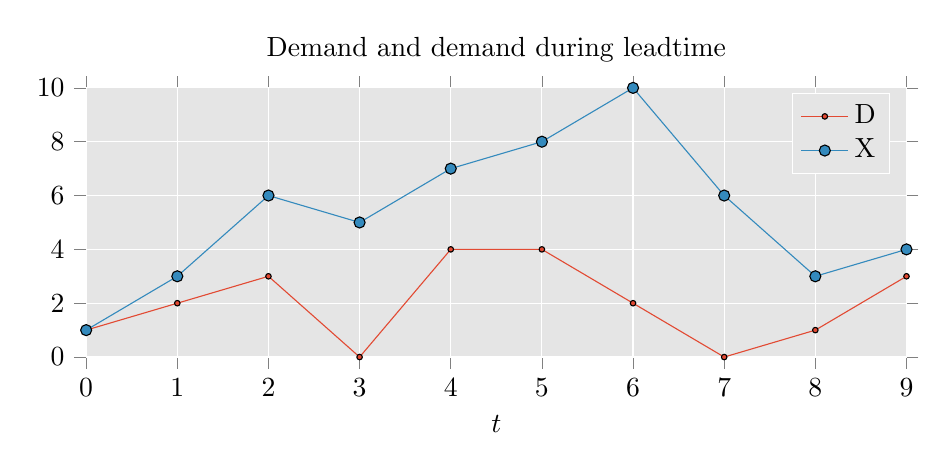
\begin{tikzpicture}

\definecolor{color0}{rgb}{0.886274509803922,0.290196078431373,0.2}
\definecolor{color1}{rgb}{0.203921568627451,0.541176470588235,0.741176470588235}

\begin{axis}[
title={Demand and demand during leadtime},
xlabel={$t$},
xmin=0, xmax=9,
ymin=0, ymax=10,
width=12cm,
height=5cm,
tick align=outside,
xmajorgrids,
x grid style={white},
ymajorgrids,
y grid style={white},
axis line style={white},
axis background/.style={fill=white!89.803921568627459!black},
legend style={draw=white, fill=white!89.803921568627459!black},
legend entries={{D},{X}},
legend cell align={left}
]
\addplot [color0, mark=*, mark size=1, mark options={solid,draw=black}]
table {%
0 1
1 2
2 3
3 0
4 4
5 4
6 2
7 0
8 1
9 3
};
\addplot [color1, mark=*, mark size=2, mark options={solid,draw=black}]
table {%
0 1
1 3
2 6
3 5
4 7
5 8
6 10
7 6
8 3
9 4
};
\end{axis}

\end{tikzpicture}\\
% % This file was created by matplotlib2tikz v0.6.0.
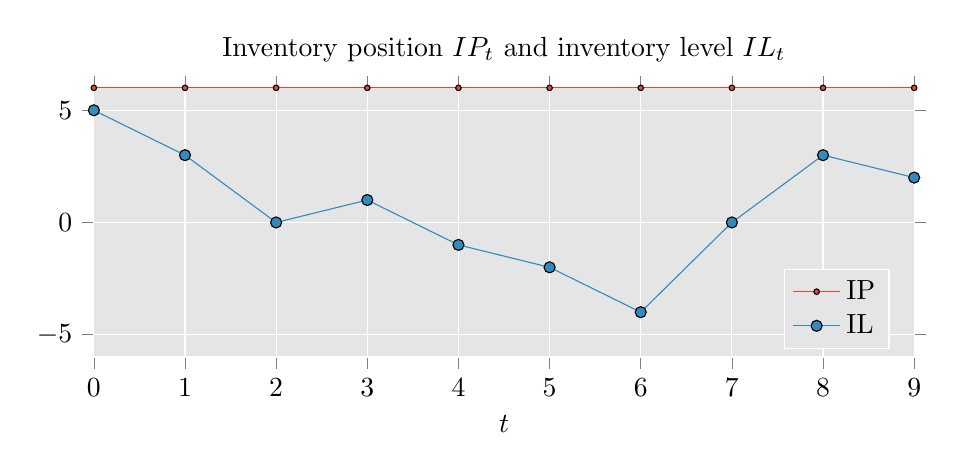
\begin{tikzpicture}

\definecolor{color0}{rgb}{0.886274509803922,0.290196078431373,0.2}
\definecolor{color1}{rgb}{0.203921568627451,0.541176470588235,0.741176470588235}

\begin{axis}[
title={Inventory position $IP_t$ and inventory level $IL_t$},
xlabel={$t$},
xmin=0, xmax=9,
ymin=-6, ymax=6,
width=12cm,
height=5cm,
tick align=outside,
xmajorgrids,
x grid style={white},
ymajorgrids,
y grid style={white},
axis line style={white},
axis background/.style={fill=white!89.803921568627459!black},
legend entries={{IP},{IL}},
legend cell align={left},
legend style={at={(0.97,0.03)}, anchor=south east, draw=white, fill=white!89.803921568627459!black}
]
\addplot [color0, mark=*, mark size=1, mark options={solid,draw=black}]
table {%
0 6
1 6
2 6
3 6
4 6
5 6
6 6
7 6
8 6
9 6
};
\addplot [color1, mark=*, mark size=2, mark options={solid,draw=black}]
table {%
0 5
1 3
2 0
3 1
4 -1
5 -2
6 -4
7 0
8 3
9 2
};
\end{axis}

\end{tikzpicture}\\
% % This file was created by matplotlib2tikz v0.6.0.
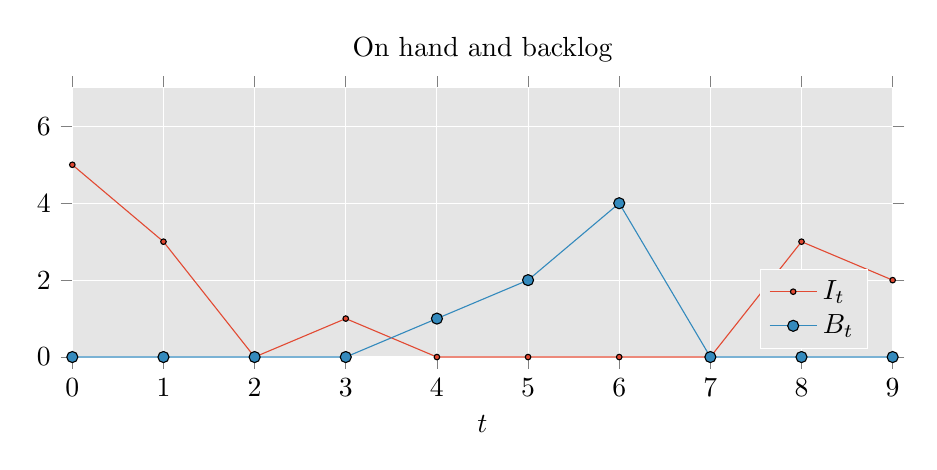
\begin{tikzpicture}

\definecolor{color0}{rgb}{0.886274509803922,0.290196078431373,0.2}
\definecolor{color1}{rgb}{0.203921568627451,0.541176470588235,0.741176470588235}

\begin{axis}[
title={On hand and backlog},
xlabel={$t$},
xmin=0, xmax=9,
ymin=0, ymax=7,
width=12cm,
height=5cm,
tick align=outside,
xmajorgrids,
x grid style={white},
ymajorgrids,
y grid style={white},
axis line style={white},
axis background/.style={fill=white!89.803921568627459!black},
legend entries={{$I_t$},{$B_t$}},
legend cell align={left},
legend style={at={(0.97,0.03)}, anchor=south east, draw=white, fill=white!89.803921568627459!black}
]
\addplot [color0, mark=*, mark size=1, mark options={solid,draw=black}]
table {%
0 5
1 3
2 0
3 1
4 0
5 0
6 0
7 0
8 3
9 2
};
\addplot [color1, mark=*, mark size=2, mark options={solid,draw=black}]
table {%
0 0
1 0
2 0
3 0
4 1
5 2
6 4
7 0
8 0
9 0
};
\end{axis}

\end{tikzpicture}
%   \end{tabular}
% \end{center}
\end{solution}
\end{exercise}




\begin{comment}
  Exercises on systems with loss
\end{comment}


\subsection{Analytic Results}

In this section we establish a set of formulas by which we can compute several performance measures as a function of the reorder level $r$. 

First, for the ready rate we have that
\begin{equation}
  \label{eq:13}
   S_r(r) = \P{\IL_i > 0} = F(r),
\end{equation}
where $F$ is defined by~\eqref{eq:16} and where we require that $i>L$ so that initial effects of the inventory no longer play a role. 


\begin{exercise}
Derive the above.
\begin{solution}
\begin{align*}
   S_r(r) &= \P{\IL_i >0} \\
   &= \P{r+1 - D[i-L, i] >0}, &\text{by \eqref{eq:b2}}  \\
   &= \P{D[i-L, i] <  r+1} \\
   & = \P{D[i-L, i] \leq  r}\\
   & = F(r)  &\text{by~\eqref{eq:16}}.
\end{align*}
\end{solution}
\end{exercise}


\begin{exercise}\label{q:basestock}
What is $S(r)$ for $r=0, \ldots, 5$ when the demand during the leadtime is given by
  \begin{align*}
    f(0) &= 1/6, & F(0) &= 1/6,  \\
    f(1) &= 1/5, & F(1)  &= 11/30,  \\
    f(2)&= 1/4, & F(2) &= 37/60, \\
    f(3) &= 1/8, & F(3)&= 89/120, \\
    f(4) &= 11/120, & F(4) &= 5/6, \\
    f(5) &= 1/6, & F(1)  &= 1.
  \end{align*}

\begin{solution}
\begin{align*}
  r &= 0 \implies S(0) = F(0) = 1/6, \\
  r &= 1 \implies S(1) = F(1) = 11/33, \\
  r &= 2 \implies S(2) = F(2) = 37/60,\\
  r &= 3 \implies S(3) = F(3) = 89/120, \\
  r &= 4 \implies S(4) = F(4) = 5/6, \\
  r &= 5 \implies S(5) = 1.
\end{align*}
\end{solution}
\end{exercise}

Next we compute the average backorder level. 

\begin{exercise}
Explain that $B_i = (D[i-L, i] - r - 1)^+$; hence a backorder only occurs  when $D[i-L, i] - r-1>0$. 
\begin{solution} Its easy to make an off-by one error. Hence, we deal with the statement in full rigor.
  \begin{align*}
    B_i 
&= I_i^- \\
&= (r+1-D[i-L, i])^- &\text{by~\eqref{eq:b2}}\\
&= (D[i-L, i]-r-1)^+.
  \end{align*}
\end{solution}
\end{exercise}

With the result of the previous exercise we can  the expected demand in backlog can be computed with the formula
  \begin{equation}  \label{eq:12}
     B(r) = \E{B_i} =\sum_{i=r+1}^\infty (i- r -1)f_i.
  \end{equation}

\begin{exercise}
Show \eqref{eq:12}. 
  \begin{solution}
\begin{align*}
     B(r) 
   &= \E{B_i} \\
   &= \E{( D[i-L, i]- r - 1)^+} \\
   &= \sum_{i=r+1}^\infty (i- r -1)\P{D[i-L, i] = i}\\
   &= \sum_{i=r+1}^\infty (i- r -1)f_i \\
   &= \sum_{i=r+2}^\infty (i- r -1)f_i,
\end{align*}
where the last equation follows from the fact that $i-r-1=0$ when $i=r+1$.
  \end{solution}
\end{exercise}

\begin{exercise}\label{q:basestock_B}
  Suppose the demand is given by  Exercise~\ref{q:basestock}. What is $B(r)$ for $r=0,\ldots, 5$.?
\begin{solution}
  Use that $B(r) = \sum_{i=r+1}^\infty (i-r-1)f(i)$, and that $f(i)=0$ for $i\geq 6$.
  \begin{align*}
    r&=0 \implies B(0) = \sum_{i=1}^\infty (i-1)f(i) =  0\cdot 1/5 + \cdots + 4 \cdot 1/6 = 173/120, \\
    r&=1 \implies B(1) = \sum_{i=2}^6 (i-2)f(i) =  1\cdot 1/8 + 2\cdot 11/120 + 3 \cdot 1/6 = 97/120, \\
    r&=2 \implies B(2) = 1\cdot 11/120 + 2 \cdot 1/6 = 17/40, \\
    r&=3 \implies B(3) = 1 \cdot 1/6 = 1/6, \\
  \end{align*}
\end{solution}
\end{exercise}

Note that in the above formula for $B(r)$ the summation runs to $\infty$, which is sometimes a bit problematic for numerical purposes. It turns out that~\eqref{eq:12} can be rewritten to 
\begin{equation} \label{eq:17}
   B(r) = \theta - \sum_{j=0}^{r} G(j)
\end{equation}
where
\begin{equation*}
    G(j) = 1 - F(j) = \P{D[i-L, i] > j},
\end{equation*}
and $\theta=\E{D[i-L, i]}$ is the average leadtime demand.

\begin{exercise}[\faRocket]
Derive~\eqref{eq:17}.
\begin{solution}
Note  that
\begin{equation*}
  \sum_{j=0}^\infty \1{j< i-r - 1} = i-r -1.
\end{equation*}
With this,
\begin{align*}
       B(r) &= 
   \sum_{i=r+1}^\infty (i-r-1) f(i)   \\
   &= \sum_{i=r+1}^\infty\sum_{j=0}^\infty \1{j < i-r-1}\, f(i)   = 
    \sum_{j=0}^\infty \sum_{i=r+1}^\infty \1{i > j +r + 1}\, f(i)\\
   &= \sum_{j=0}^\infty \sum_{i=j + r+2}^\infty  f(i) = 
   \sum_{j=0}^\infty \P{D[k-L, k] \geq j + r+2}  &\text{ for any } k \\
   &=\sum_{j=0}^\infty \P{D[k-L, k] > j + r+1} \\
   &= \sum_{j=r+1}^\infty  G(j).
\end{align*}
This can be simplified a bit further by using that
$\sum_{i=0}^\infty \bar G(i) = \theta$:
\begin{align*}
   B(r) 
   &= \sum_{j=r+1}^\infty  G(j) \\
   &= \sum_{j=0}^\infty  G(j) - \sum_{j=0}^{r} G(j)\\
   &= \theta - \sum_{j=0}^{r} G(j)
\end{align*}
\end{solution}
\end{exercise}
	   
\begin{exercise}What is $\theta$ for the demand of Exercise~\ref{q:basestock}?
\begin{solution}
  \begin{align*}
    \theta = \E{X} =
0\cdot \frac 1 6 + 1\cdot \frac 1 5 + \cdots + 5 \cdot \frac 1 6 = \frac{91}{40}.
  \end{align*}
\end{solution}
\end{exercise}

\begin{exercise}
  Show that the results of \eqref{eq:12} and \eqref{eq:17} coincide for the data of Exercise~\ref{q:basestock}.
\end{exercise}


Finally, by taking expectations at the left and right hand side of~\eqref{eq:b2} and using \eqref{eq:2a} it follows that for the average on-hand inventory 
\begin{equation}\label{eq:19}
I(r) = \E{\IL_i^+} = r+1 - \theta + B(r)
\end{equation}

\begin{exercise}
Derive \eqref{eq:19}. 
\begin{solution} We can use \eqref{eq:3} and \eqref{eq:4} to see that $\IL_i^+ - \IL_i^- = \IL_i$. Next, since $\IL_i = r+1 - D[i-L, i]$, we have that 
  \begin{equation*}
    \IL_i^+ = \IL_i + \IL_i^-=r+1 - D[i-L, i] + \IL_i^-.
  \end{equation*}
Taking expectations and recalling that $B_i = \IL_i^+$,
\begin{align*}
  \E{\IL_i^+}
  &= r+1 - \E{D[i-L, i]} + \E{B_i}  \\
  & = r + 1 - \theta + B(r).
\end{align*}
\end{solution}
\end{exercise}

\begin{exercise}
Suppose the demand is given by Exercise~\ref{q:basestock}. What is $I(r)$ for $r=0,\ldots, 5$.?

\begin{solution}
 The result follows straightaway from Exercise~\ref{q:basestock_B}. As an example
  \begin{equation*}
    I(3) = 3+1 - \theta + B(3) = 4 - 91/40 + 1/6 = 227/120.
  \end{equation*}
\end{solution}
\end{exercise}

\begin{exercise}
Suppose the demand is given by the previous exercise and that the holding cost $h=1$ and the backlog cost per item is $b=5$.  Which value for $r$ minimizes $h I(r)+b B(r)$?
\nvf{To be done}
\end{exercise}

\nvf{Do we still want to skip these formulas?} Formulas to skip (in FP edition 3): 2.24, 2.25. 

\nvf{Make the stuff for normally distributed demand, also for the q,r model?}

\Closesolutionfile{ans}
\opt{solutionfiles}{
\subsection{Solutions}
\input{ans}
}

\clearpage
%%% Local Variables:
%%% mode: latex
%%% TeX-master: "inventory_notes"
%%% End:



% 
\subsection{$(Q,r)$ Model}

\subsubsection{Computing the service level}

The service level is
\begin{equation}
  \label{eq:5}
  \begin{split}
   S(Q,r) 
   &= \frac1Q \sum_{i=r}^{r+Q-1} S(i) \\
   &= \frac1Q \sum_{i=r}^{r+Q-1} G(i),
  \end{split}
\end{equation}
where $S(i)$ is the service level of the basestock model with reorder
level $i$, i.e. $S(i)=G(i)$ is given by \eqref{eq:13}.  To verify that
the summation should start at $r$, and not at $r+1$ (as I have found
somewhere), we can take $Q=1$, as then the $(Q,r)$ model reduces to
the basestock model. The above formula then gives $S(1,r)= G(r)$, and
this is the same formula as found for the basestock model, i.e.,
\eqref{eq:13}.


Factory Physics mentions also the following formula:
\begin{equation}
  \label{eq:1}
   S(Q,r) = 1- \frac1Q [B(r-1) - B(r+Q-1)],
\end{equation}
where $B(r)$ can be computed according to \eqref{eq:12}.  I find
expression \eqref{eq:5} conceptually more important than \eqref{eq:1}. 

\begin{remark}
  
It
appears that in Eq. 2.70 of FP, edition 3, are is off by one. To see
this, we prove that \eqref{eq:1} is indeed the same as \eqref{eq:5}. It
follows from \eqref{eq:1} and \eqref{eq:5} that
\begin{equation*}
  \begin{split}
   B(r-1) - B(r+Q-1) 
   &= Q - Q S(Q,r) \\
   &= Q - \sum_{i=r}^{r+Q-1} S(i) \\
   &= \sum_{i=r}^{r+Q-1}(1- S(i)) \\
   &= \sum_{i=r}^{r+Q-1}(1- G(i)),
  \end{split}
\end{equation*}
since $\sum_{i=r}^{r+Q-1} 1 = Q$. From \eqref{eq:13} we see that $S(i)
= G(i)$. With \eqref{eq:18} this becomes
\begin{equation*}
  \begin{split}
    B(r-1) - B(r+Q-1)
    &= \sum_{i=r}^{r+Q-1}(1- G(i))\\
    &= \sum_{i=r}^{r+Q-1} \bar G(i)\\
    &= \sum_{i=r}^{\infty} \bar G(i) -\sum_{i=r+Q}^\infty \bar G(i).
  \end{split}
\end{equation*}
From \eqref{eq:19} it follows that $B(r-1)=\sum_{i=r}^{\infty} \bar
G(i)$, and likewise for $B(r-1+Q)$. We are done.
\end{remark}

\subsubsection{Computing  backorders}

The expected number of back-orders is 
\begin{equation}
  \label{eq:14}
   B(Q,r) = \frac1Q \sum_{i=r}^{r+Q-1} B(i),
\end{equation}
where $B(i)$ is defined in \eqref{eq:12}. To convince ourselves
that the summation has to start at $r$, observe that for
$Q=1$, we get \eqref{eq:12} of the basestock model.


\subsubsection{Expected Inventory Level}

The expected inventory level can be found as follows. Let $I(r)$
be the long-run time average inventory level, i.e., \eqref{eq:6}. Then,

\begin{equation}\label{eq:2}
  \begin{split}
   I(Q,r)
   &= \frac1Q\sum_{i=r}^{r+Q-1} I(i) \\
   &= \frac1Q\sum_{i=r}^{r+Q-1} (i+1 - \theta + B(r)) \\
   &= \frac1Q\sum_{i=r}^{r+Q-1} (i + 1)  - \theta + \frac1Q\sum_{i=r}^{r+Q-1} B(r) \\
   &= \frac{Q+1}2 + r - \theta + B(Q,r), 
  \end{split}
\end{equation}
where we use \eqref{eq:14}. What do you get when $Q=1$?

Formulas to skip (in edition 3): 2.38, 2.41, 2.42, 2.43.

\begin{question}
  Take the data from Exercise~\ref{q:basestock}. Suppose $r=1$ and $Q=2$. What is $S(Q,r)$?
\end{question}
\begin{solution}
  Use~\eqref{eq:5}.
  \begin{equation*}
    \begin{split}
      S(2,1)
&= \frac{1}Q\sum_{i=r}^{r+Q-1} G(i) \\
&= \frac{1}Q\sum_{i=r}^{r+Q-1} \P{X\leq i} \\
&= \frac{1}Q\sum_{i=1}^{1+2-1} \P{X\leq i} \\
&= \frac 12 \sum_{i=1}^{2} \P{X\leq i} \\
&=  \frac 12 (\P{X\leq 1} + P{X\leq 2}) \\
&= \frac12(11/30 + 37/60) = 59/120.
    \end{split}
  \end{equation*}
\end{solution}

\begin{question}
  Take the data from Exercise~\ref{q:basestock}. Suppose $r=1$ and $Q=2$. What is $B(Q,r)$?
\end{question}
\begin{solution}
Use~\eqref{eq:14} and the results of Exercise~\ref{q:basestock_B}
  \begin{equation*}
    \begin{split}
      B(2,1)
&= \frac1Q \sum_{i=r}^{r+Q-1} B(i) \\
&= \frac12 \sum_{i=1}^{2} B(i) \\
&= \frac12 (B(1) + B(2)) \\
&= \frac12 \left(\frac{97}{120} + \frac{17}{40}\right) = \frac{37}{60}.
\end{split}
\end{equation*}
\end{solution}


\begin{question}
  Take the data from Exercise~\ref{q:basestock}. Suppose $r=1$ and $Q=2$. What is $I(Q,r)$?
\end{question}
\begin{solution}
  Use~\eqref{eq:2} and the previous exercise and the result of Exercise~\ref{q:basestock_theta}.

  \begin{equation*}
    I(2,1)  = \frac{2+1}2 + r - \frac{91}{40}+ \frac{37}{60} = \frac{101}{120}.
  \end{equation*}
\end{solution}


\subsubsection{Simulation of the (Q,r) inventory model}

Consider a periodic-time model so that the inventory position $\IP_i$
is the inventory position at the end of period $i$. Then the sequence
$\{\IP_i\}$ must satisfy the recursion:
\begin{equation}
  \IP_i = \IP_{i-1} - D_i + Q \1{\IP_{i-1} - D_i\leq r}.
\end{equation}
To see this, observe that under the $(Q,r)$ policy the inventory
position is always kept above level $r$. Thus, if the inventory
position at the end of period $i-1$ minus the demand $D_i$ during
period $i$ is less than $r+1$, we need to place a replenishment
reorder of size $Q$.  Note that we assume here that $D_i\leq Q$ always.

When the leadtime $L$ is one period or more, the replenishments do not
arrive right away but $L$ periods later. The consequences of the
inventory level are that
\begin{equation}
  \IL_i = \IL_{i-1} - D_i + Q\1{\IP_{i-1-L} - D_{i-L}\leq r}.
\end{equation}
Compare~\eqref{eq:21} of the basestock model.

The performance measures are the same as for the basestock model discussed in Section~\ref{sec:simul-basest-invent}.


\subsubsection{Example Code}
\label{sec:qr_example-code}

Here is the code by which we computed the answers to the exercises. We include it for the interested student; feel free to skip it otherwise.

\lstinputlisting[language=Python]{basestock.py}


%%% Local Variables:
%%% mode: latex
%%% TeX-master: "notes_all"
%%% End:

% 
\subsection{Joint Ordering}

 
\begin{itemize}
\item ABC classification
\item See FP, ch 17 for other models.
\end{itemize}



%%% Local Variables:
%%% mode: latex
%%% TeX-master: "notes_all"
%%% End:


\section{Performance Analysis of Inventory Policies}
%\section{Performance Analysis of Inventory Policies}

We recommend to study the following topics (mainly in Chapter 17, but please take also a look at Chapter 2:

\begin{itemize}
\item ABC classification
\item Slow-moving items
\item Fast-moving items
\item Routine items
\item Coordinated replenishment in multi-item inventory systems
\end{itemize}

\begin{itemize}
\item Graphs
\item formulas,
\item models.
\end{itemize}

%%% Local Variables:
%%% mode: latex
%%% TeX-master: "notes_all"
%%% End:




%\bibliographystyle{plainnat}
%\bibliography{inventory}
\end{document}

%%% Local Variables:
%%% mode: latex
%%% TeX-master: t
%%% End:
